\chapter{La geometría griega}

En este capítulo hablaremos de la geometría griega. Naturalmente una parte
sustancial de este capítulo estará dedicada a los famosos trece libros de
Euclides. Si bien cada vez que sea necesario transcribir partes de los libros
de Euclides utilizaremos una traducción al castellano hecha por María Luisa
Puertas Castaño~\cite{elementos1,elementos2}, quizá sea oportuno remarcar que el interesado en un estudio
histórico más profundo de la matemática contenida en estos libros de Euclides
deberá consultar la excelente versión de los libros de Euclides traducida y
comentada por el historiador de la matemática (y además experto en la
matemática griega) Thomas Heath~\cite{MR1932864}. 

Para los griegos, la geometría era la rama más importante de la matemática.
Alrededor del 300 a. C. Euclides organizó gran parte de la matemática que se
conocía en aquel momento y escribió trece libros.  El tratado de Euclides fue
el texto más influyente en la historia de la matemática y fue fundamental quizá
hasta principios del siglo XX. 

Es poco lo que se conoce de la matemática anterior a la época de Euclides. En
sus comentarios sobre los elementos de Euclides, Proclo hace un breve resumen
histórico; muy posiblemente este resumen esté fuertemente basado en un tratado
sobre historia de la matemática escrito por Eudemo. Proclo menciona que muchos
autores atribuyen a los egipcios la invención de la geometría, nacida para
atacar problemas prácticos tales como la medición de campos. Proclo además
afirma que los fenicios fueron los primeros en tener un conocimientos de los
números debido a las transacciones comerciales. Según Proclo, Tales estuvo en
egipto y fue el primero en llevar la geometría a Grecia. El estudio sistemático
de la geometría, con teoremas abstractos que se obtienen a partir de principios
generales, se le atribuye a los miembros de la escuela de Pitágoras. Platón
mostró gran interés en la geometría y justamente eso fue lo que le dio un
impulso extraordinario.

%A Tales se le atribuyen varias constribuciones geométricas fundamentales, por ejemplo que todo diámetro biseca a la circunferencia, 
%que los ángulos de la base de un triángulo isósceles son iguales, que ángulos opuestos por el vértice son iguales, y la resolución
%de varios problemas de aplicación como el de calcular la distancia entre una nave y el puerto, o calcular
%la altura de una pirámide sabiendo cuánto mide la sombra que proyecta. 
%El resultado que hoy conocemos como el teorema de Tales aparece en el libro VI de los elementos. 

Los libros de Euclides comienzan con definiciones (que para nosotros quizá no
siempre resultan del todo precisas). Por ejemplo, el \emph{punto} se define
como lo que no tiene partes; esta es la primera definición. La segunda
definición dice que una \emph{línea} es una longitud sin anchura. La tercera,
que los extremos de una línea son puntos. (Hay que aclarar que estas
definiciones fueron tomadas de la traducción de los elementos hecha por Puertas
Castaño.) Figuran en los libros de Euclides 
además las definiciones de círculo, ángulos rectos y agudos,
etc.

Después de las definiciones, se presentan los postulados. El primero de los
postulados afirma que siempre existe una línea recta que une dos puntos
distintos del plano. En mi traducción\footnote{La versión de los Elementos que
	se utilizará en este curso, y en particular durante este capítulo, es una
	edición la editorial Gredos, con traducción y notas de María
Luisa Puertas Castaños.}, leo la siguiente oración: 
\begin{quote}
	Postúlese el trazar una línea recta dado un punto cualquiera hasta un punto
	cualquiera. 
\end{quote}
El segundo postulado afirma que es posible prolongar continuamente una recta
finita en línea recta; es decir: se afirma que una línea puede extenderse tanto
como sea necesario en cualquiera de las dos direcciones posibles.  El tercer
postulado afirma que dado un punto $P$ y una distancia $r$, puede construirse
un círculo con centro en $P$ y radio $r$. Uno de estos postulados, el quinto,
es particularmente importante dentro del desarrollo histórico de la matemática: 

\begin{quote}
	Si una recta al incidir sobre dos rectas hace los ángulos internos del
	mismo lado menores que dos rectos, las dos rectas prolongadas
	indefinidamente se encontrarán en el lado en el que estén los (ángulos)
	menores que dos rectos.
\end{quote}

En este postulado se basa un hecho notable: la geometría de los libros de
Euclides no es sino una de las geometrías posibles. Es sorprendente que
Euclides haya considerado necesario incluir este quinto postulado para fijar
condiciones que garanticen que dos rectas se corten en un único punto.  Más de
dos mil años después de aquella genialidad, al reemplazar este postulado la
matemática encontrará geometrías distintas a la geometría estudiada por
Euclides, las denominadas geometrías no euclidianas.

Además de los postulados hay doce \emph{nociones comunes}. La primera de estas
nociones comunes afirma que \emph{las cosas iguales a una misma cosa son
también iguales entre sí}. En nuestro lenguaje algebraico, esto equivale a que
si $A=B$ y además $A=C$, entonces $B=C$.  

A partir de esas definiciones básicas, de los axiomas y los postulados,
Euclides desarrolló la geometría. Por ejemplo, la primera proposición del libro
I explica cómo construir un triángulo equilátero sobre una recta finita dada.
La proposición es acompañada por una figura similar a la
figura~\ref{fig:libroI_prop1}. 

\begin{figure}
   \centering
   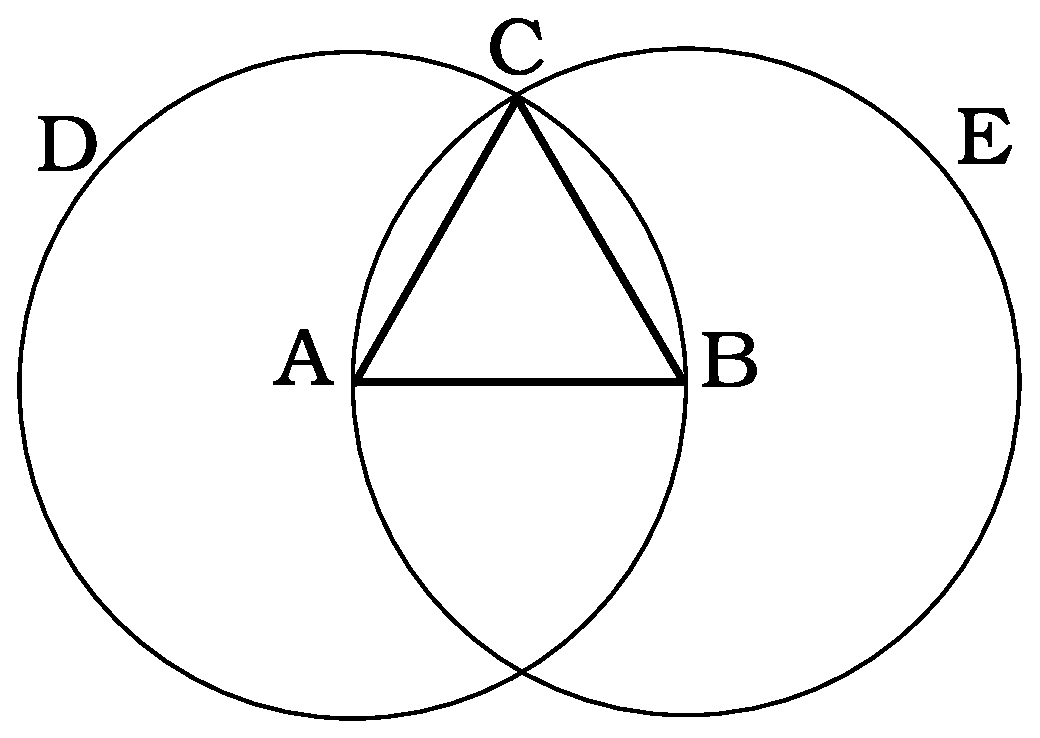
\includegraphics[scale=0.2]{images/libroI_prop1}
   \caption{La proposición 1 del libro I.}
   \label{fig:libroI_prop1}
\end{figure}

La demostración es breve y sencilla, aunque no es del todo convincente pues
faltan justificaciones. Es la primera demostración de los libros de Euclides, y
quizá por eso acumula muchas más críticas que las otras demostraciones.  

La proposición 47 del libro I es el teorema de Pitágoras: 
\begin{quote}
	En los triángulos rectángulos el cuadrado del lado que subtiende el ángulo
	recto es igual a los cuadrados de los lados que comprenden el ángulo recto.
\end{quote}
Se cree que la demostración basada en la figura~\ref{fig:libroI_prop47} fue
descubierta por Euclides.


\begin{figure}
   \centering
   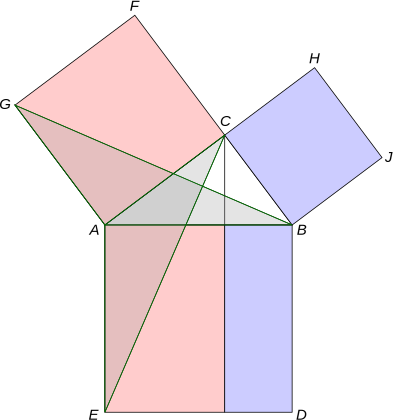
\includegraphics[scale=0.4]{images/libroI_prop47}
   \caption{La demostración del teorema de Pitágoras dada por Euclides.}
   \label{fig:libroI_prop47}
\end{figure}

En el segundo libro aparecen ciertas nociones algebraicas, aunque en un
lenguaje completamente distinto al que usamos en estos tiempos. La primera
proposición de este libro, por ejemplo, afirma lo siguiente: 
\begin{quote}
	Si hay dos rectas
	y una de ellas se corta en un número cualquiera de segmentos, el rectángulo
	comprendido por las dos rectas es igual a los rectángulos comprendidos por la
	(recta) no cortada y cada uno de los segmentos.
\end{quote}
Nuestra notación algebraica
nos permite reconocer en esta proposición la propiedad distributiva: 
\[
	a(b+c+\cdots)=ab+ac+\cdots
\]
La cuarta proposición afirma lo siguiente: 

\begin{quote}
	Si se corta al azar una línea recta,
	el cuadrado de la (recta) entera es igual a los cuadrados de los segmentos y
	dos veces el rectángulo comprendido por los segmentos.
\end{quote}
Esta proposición puede traducirse de la siguiente forma:
\[
	(a+b)^2=a^2+2ab+b^2.
\]

Las proposiciones 12 y 13 del libro II contienen resultados similares al
teorema del coseno, aunque sin hacer uso de funciones trigonométricas. La
trigonometría se desarrolló algún tiempo después de que Euclides escribió sus
Elementos. 

%Veamos otro resultado, ahora del tercer libro.  La proposición 35 del libro III
%afirma lo siguiente: 
%
%\begin{quote}
%Si en un círculo se cortan dos rectas entre sí, el
%rectángulo comprendido por los segmentos de una es igual al rectángulo
%comprendido por los segmentos de la otra.
%\end{quote}
%
%En lenguaje moderno esta proposición puede enunciarse de la siguiente forma: 

Recordemos que los griegos no podían medir distancias pero sí sabían cómo
comparar segmentos y reconocer cuándo dos segmentos son iguales o cuándo uno
es, digamos, el doble de otro. Los griegos tampoco podían medir ángulos. Gran
parte de la manera de pensar de los griegos era geométrica. Para ellos lo que
ahora sería el producto $ab$ entre los números $a$ y $b$ era simplemente el
área de un rectángulo de lados $a$ y $b$. La ecuación $ab=cd$ era interpretada
entonces como la igualdad entre las áreas de ciertos rectángulos.

En los libros de euclides hay además construcciones explícitas con regla y
compás, aunque Euclides en ningún momento hace referencia a estos u otros
instrumentos geométricos. 

\begin{exercise}
	Construya con regla y compás el punto medio de un segmento.
\end{exercise}

El mismo truco permite también construir un triángulo equilátero si uno de los
lados está dado.

\begin{exercise}
	Construya con regla y compás un cuadrado.	
\end{exercise}

Una pregunta interesante es la siguiente: ¿cómo puede construirse con regla y
compás un pentágono regular? Euclides dio una construcción.

\begin{exercise}
	Construya un pentágono regular con regla y compás. 
\end{exercise}

Es natural preguntarse cómo puede construirse o hexágono regular o, más
generalmente, cualquier $n$-ágono regular. Construir un hexágono es fácil ya
que sabemos construir triángulos equiláteros. Sin embargo, no puede construirse
un heptágono regular con regla y compás. Sí podemos, en cambio, construir un
octágono. 

En 1796 Gauss pudo construir con regla y compás un polígono regular de $17$
lados. Gauss no solamente encontró la forma de construir ese polígono regular
sino que demostró además que un polígono regular de $n$ lados puede construirse
con regla y compás sí y sólo si $n=2^mp_1\cdots p_k$ con $p_1,\dots,p_k$ primos
de Fermat distintos. Los primos de la forma 
\[
	p=2^{2^l}+1
\]
se conocen como \textbf{primos de Fermat}. Hasta el momento los únicos primos
de Fermat conocidos son los siguientes:
\[
	3,5,17,257,65537.
\]
Y se conjetura que esos son los únicos primos de Fermat que existen. Para más
información acerca de los primos de Fermat referimos a
las sucesiones 
\href{https://oeis.org/A000215}{A000215}.
y \href{https://oeis.org/A019434}{A019434}.

\index{Problema!de la trisección del ángulo}
\index{Problema!de la cuadratura del círculo}
\index{Problema!de la duplicación del cubo}
Las construcciones con regla y compás ocupaban un lugar importante en el
pensamiento de los geómetras griegos. Los griegos sabían cómo construir
$\sqrt{2}$ e incluso cómo construir $\sqrt{n}$ para cualquier $n$. Sin embargo,
no sabían cómo construir $\sqrt[3]{2}$; este problema se conoce como el
\textbf{problema de la duplicación del cubo}, ya que el problema consiste en
duplicar el volumen de un cubo dado). Otros problemas similares que mucho
interesaban a los griegos son los siguientes: el
\textbf{problema de la trisección de un ángulo} y el \textbf{problema de la
cuadratura del círculo} (en este problema se pide construir un cuadrado de área
igual al área de un círculo dado, o bien, equivalentemente, construir $\pi$).

Los pitagóricos habían resuelto el problema de la cuadratura de los polígonos.
Antifón demostró que dado un polígono inscrito en un círculo, siempre se puede
duplicar la cantidad de lados del polígono. De esto, concluyó erroneamente que
el círculo es cuadrable ya que puede aproximarse con arbitraria precisión por
polígonos cuadrables. Aristóteles observó que estos polígonos jamás llenarán al
círculo, sin importar qué tan grande sea el número de lados empleado. Tiempo
más tarde, Brisón mejoró el argumento y consideró sucesiones de polígonos
inscritos y circunscritos que aproximan cada vez mejor al círculo. Esta idea
fue retomada muy exitosamente por Arquímedes en sus trabajos sobre
aproximaciones del número $\pi$. Hipócrates redujo el problema de la cuadratura
del círculo a un problema de geometría plana. Si bien no logró resolver
complemente el problema de la cuadratura del círculo, sí logró cuadrar ciertos
recintos limitados por arcos, algo que hoy conocemos como \emph{lúnulas de
Hipócrates}

\begin{figure}
   \centering
   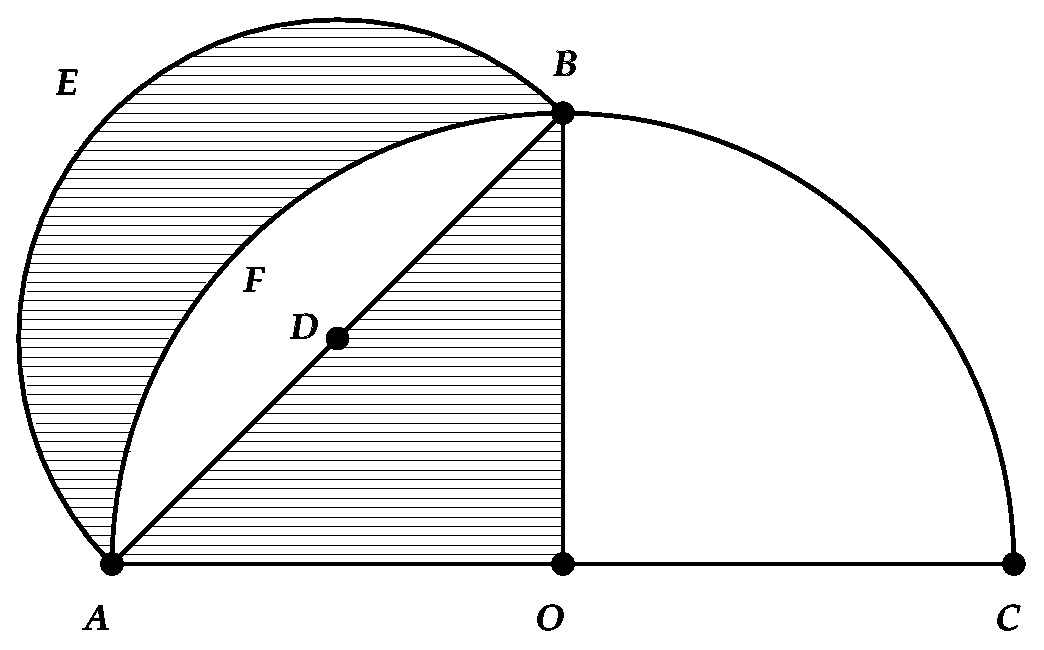
\includegraphics[scale=0.3]{images/lunula}
   \caption{Las lúnulas de Hipócrates.}
   \label{fig:lunula}
\end{figure}

\index{Lúnulas de Hipócrates}
Hipócrates probó que las áreas
sombreadas que vemos en la figura~\ref{fig:lunula} coinciden. La demostración del
resultado sobre lúnulas de Hipócrates es más o menos así: Sabemos que $D$ es el
centro del círculo que incluye el arco $AEB$, y es también el punto medio entre $A$
y $B$, que es la hipotenusa del triángulo $ABO$. Como $ABO$ es rectángulo e
isósceles, el diámetro $AC$ del círculo grande es $\sqrt{2}$ veces el tamaño del
diámetro del círculo que incluye al arco $AEB$. Como el área del círculo que
incluye al arco $ABC$ es la mitad del área del círculo que incluye al arco $AEB$,
entonces el área del cuarto de círculo $AFBOA$ es igual al área del semicírculo
$AEBDA$. Esto implica que las áreas sombreadas coinciden ya que ambas se obtienen
al restar el $AFBDA$ de regiones con la misma área. 

%Lamentablemente, el libro de Hipócrates se perdió, pero muy posiblemente haya
%servido de modelo para los Elementos de Euclides.

\begin{exercise}
	¿En qué consiste el problema de la trisección de un ángulo?
\end{exercise}

\index{Cuadratiz de Hipias}
Hipias logró resolver el problema de la trisección de un ángulo si se admite el
uso de una curva especial, que, tal como se demostró muchos años después, 
también permite
resolver el problema de la cuadtratura del círculo. Esta curva hoy se conoce
como la \emph{cuadratiz de Hipias} y puede describirse por la siguiente
función
\[
x\mapsto x\cot\left(\frac{\pi}{2a}x\right).
\]
Una representación gráfica en el caso $a=1$ puede verse en 
la figura \ref{fig:cuadratiz}.

\begin{figure}
   \centering
   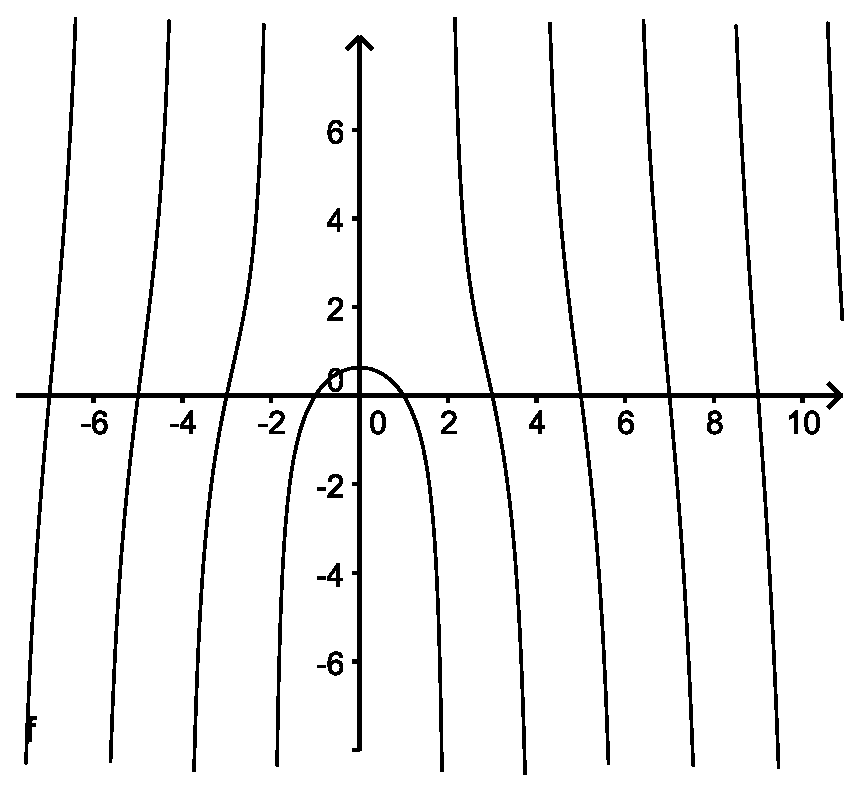
\includegraphics[scale=0.3]{images/cuadratiz}
   \caption{La cuadratiz de Hipias.}
   \label{fig:cuadratiz}
\end{figure}


% Agregar las ecuaciones y el svg de la página de wikipedia

\begin{exercise}
	¿Cómo puede construirse el número $\sqrt{n}$ con regla y compás?
\end{exercise}

\index{Número!trascendente}
\index{Número!algebraico}
\index{Número!construible}
Hoy sabemos que ninguno de estos tres problemas clásicos de la matemática
griega tiene solución. 

El problema de la duplicación del cubo y de la
trisección de un ángulo fue resuelto en 1837 por un matemático francés llamado
Pierre Wantzel. Poca gente hoy sabe que Wantzel fue el primer matemático que
fue capaz de resolver esos famosos problemas, quizá porque los métodos de
Wantzel fueron opacados por las ideas provenientes de la teoría de Galois.  

El
problema de la cuadratura del círculo fue resuelto por Lindelmann en 1882 al
demostrar que el número $\pi$ es trascendente. Un número se dice
\textbf{trascentente} si no es un número algebraico, es decir si no es raíz de
un polinomio con coeficientes racionales. Los números trascendentes, en
particular, no pueden construirse con regla y compás:
\[
	\{\text{números construibles}\}\subsetneq\{\text{números algebraicos}\}
\]

\index{Sólidos platónicos}
\index{Poliedro regular}
Otro gran descubrimiento importante para griegos es la construcción de los cinco
sólidos platónicos existentes. Un sólido platónico es un poliedro regular
convexo acotado por un cierto número de caras. Los sólidos platónicos son los
análogos espaciales de los polígonos regulares del plano. Sorprendentemente, y
a diferencia de lo que pasa con los polígonos regulares en el plano, existen
únicamente cinco poliedros regulares: el tetraedro, el cubo, el octaedro, el
dodecaedro y el icosaedro. No es difícil demostrar que, de existir poliedros
regulares, hay únicamente cinco posibilidades (y se cree que este resultado era
ya conocido por los pitagóricos). La dificultad está en demostrar que
efectivamente existen esos cinco poliedros; la dificultad está en poder
construir explícitamente esos cinco poliedros. Es fácil construir el tetraedro
o el cubo pero ¿cómo podemos construir, por ejemplo un icosaedro? Euclides no
solamente reconoció la dificultad y la belleza de este problema, sino que lo
resolvió y lo ubicó cerca del final de sus elementos. 

\begin{figure}
   \centering
   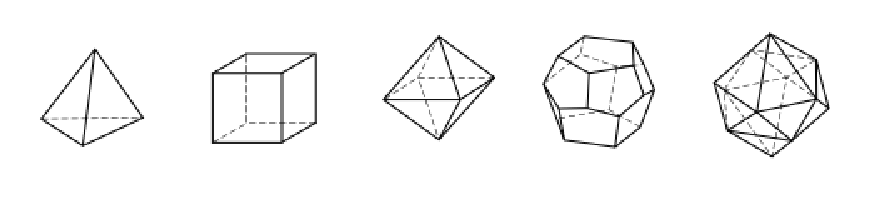
\includegraphics[scale=0.7]{images/platonic}
   \caption{Los sólidos platónicos.}
   \label{fig:platonic}
\end{figure}

Hay cierta controversia alrededor de los verdaderos descubridores de los
sólidos platónicos. La tradición nos dice los orígenes del dodecaedro, del cubo
y del octaedro están en los pitagóricos. Se nos dice además que el octaedro y
el icosaedro fueron descubiertos por Teeteto, colaborador de Platón. 

Hay gente que cree que los sólidos platónicos son muy anteriores,
creencia que se basa en la existencia de ciertas piedras del período neolítico
encontradas en Escocia, y que podemos ver en la figura~\ref{fig:piedras}. En la
opinión de Lloyd~\cite{MR2992714}, a pesar de que haber encontrado estas piedras resulte
un hecho absolutamente fascinante, 
existe poca o nula evidencia de que las piedras neolíticas de la
figura~\ref{fig:piedras} tengan alguna relación con la matemática. 
 
\begin{figure}
   \centering
   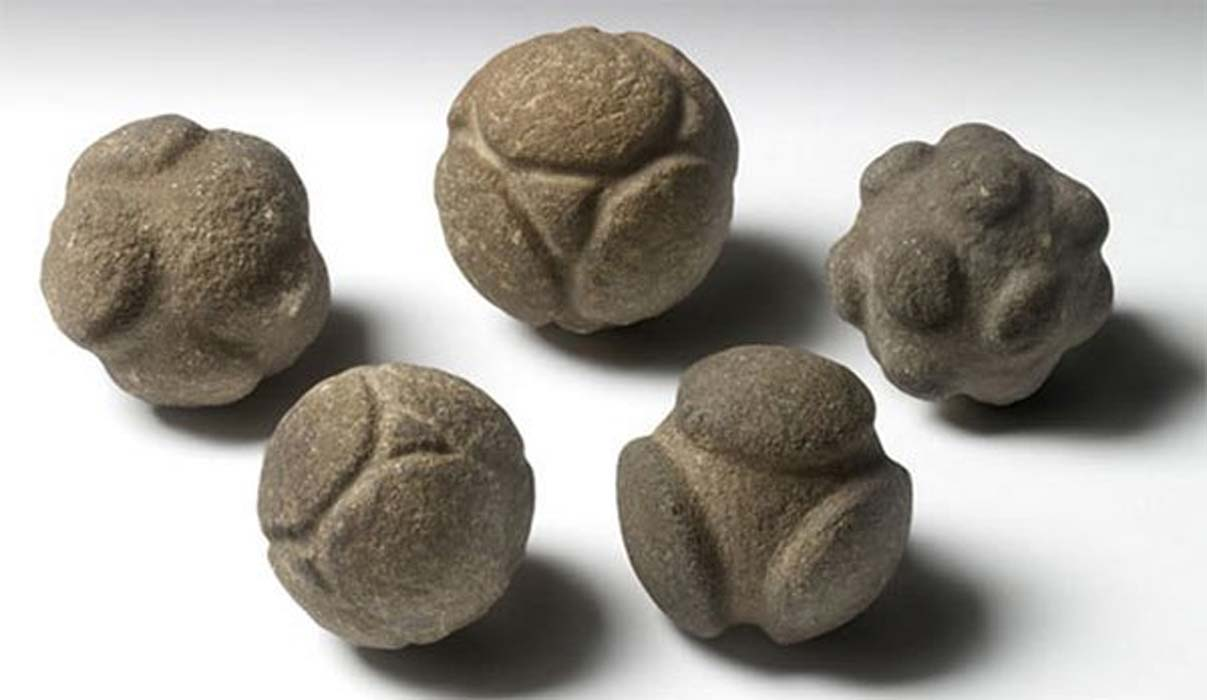
\includegraphics[scale=0.1]{images/stones}
   \caption{Piedras del período neolítico encontradas en Escocia.}
   \label{fig:piedras}
\end{figure}



En 1596 Kepler presentó una teoría sobre las distancias planetarias donde los
cinco poliedros regulares ocupan un rol fundamental. La teoría
de Kepler describe las órbitas planetarias como esferas encajadas
entre sólidos platónicos. 

\begin{figure}
   \centering
   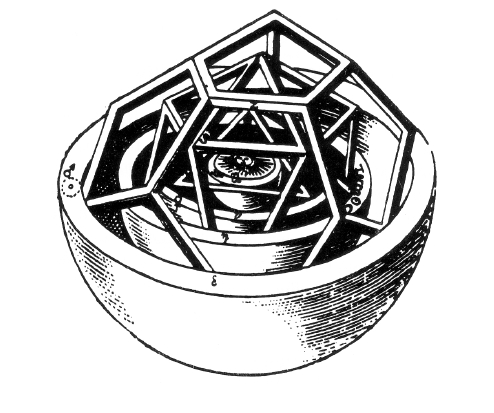
\includegraphics[scale=0.3]{images/kepler}
   \caption{La teoría de Kepler sobre órbitas planetarias.}
   \label{fig:kepler}
\end{figure}

Kepler observó que la existencia de únicamente cinco poliedros regulares era
compatible con la existencia de únicamente seis planetas. El descubrimiento de
Urano en 1781 destrozó a la teoría de Kepler. De todas formas, no fueron
necesarios otros planetas para que la teoría de Kepler perdiera valor. 

En 1609
Kepler descubrió que las órbitas planetarias son elipses; este hecho fue
explicado en 1687 por la teoría gravitatoria de Newton. 



\begin{exercise}
	En 1509 Luca Pacioli presentó una ingeniosa construcción del icosaedro
	basada en la figura~\ref{fig:Pacioli}.  ¿Cuál es esa construcción?
\end{exercise}

\begin{figure}
   \centering
   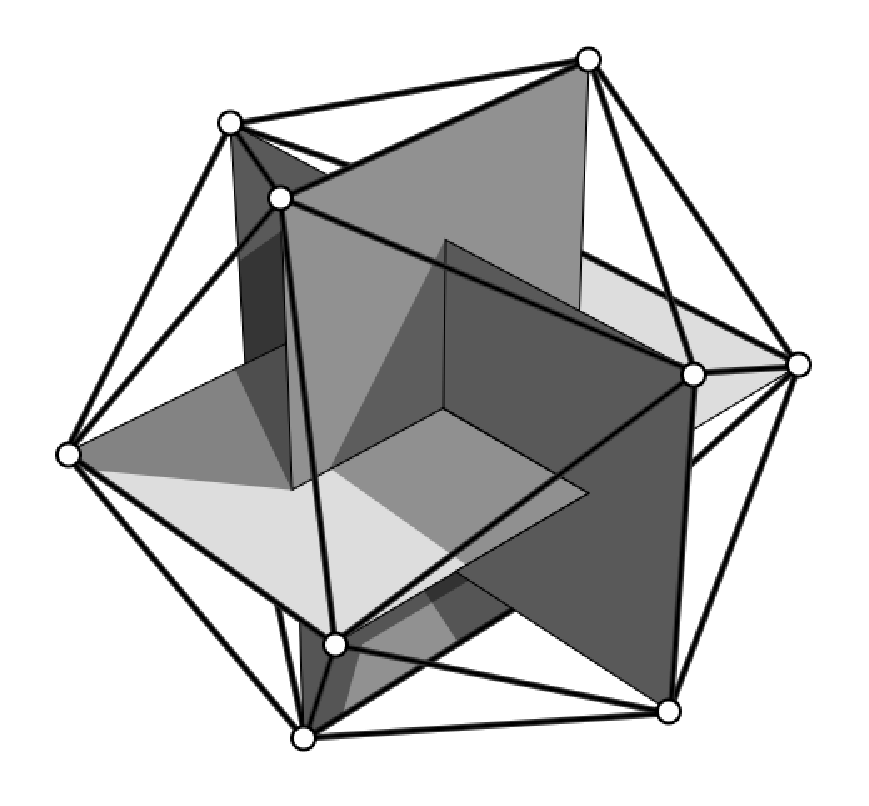
\includegraphics[scale=0.3]{images/pacioli}
   \caption{La construcción del icosaedro de Pacioli.}
   \label{fig:Pacioli}
\end{figure}

\index{Rectángulo áureo}
\index{Número!áureo}
La construcción del icosaedro dada por Pacioli utiliza rectángulos áureos. Un
rectángulo áureo es un rectángulo como el que vemos en la
figura~\ref{fig:golden} donde 
\[
	\frac{a+b}{a}=\frac{a}{b}.
\]

\begin{figure}
   \centering
   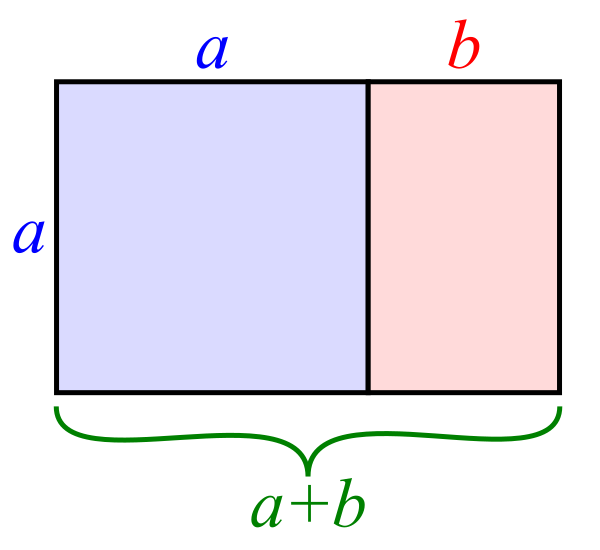
\includegraphics[scale=0.2]{images/golden}
   \caption{El rectángulo áureo.}
   \label{fig:golden}
\end{figure}

Puede demostrarse que el cociente $a/b$ es entonces solución de la ecuación
cuadrática $x^2-x-1=0$ y luego 
\[
	a/b=\frac{1+\sqrt{5}}{2}=1,6180339887\cdots,
\]
número que comunmente se denota con la letra griega $\varphi$.  La
figura~\ref{fig:construction} nos muestra que el número $\varphi$ es
construible con regla y compás. 

\begin{figure}
   \centering
   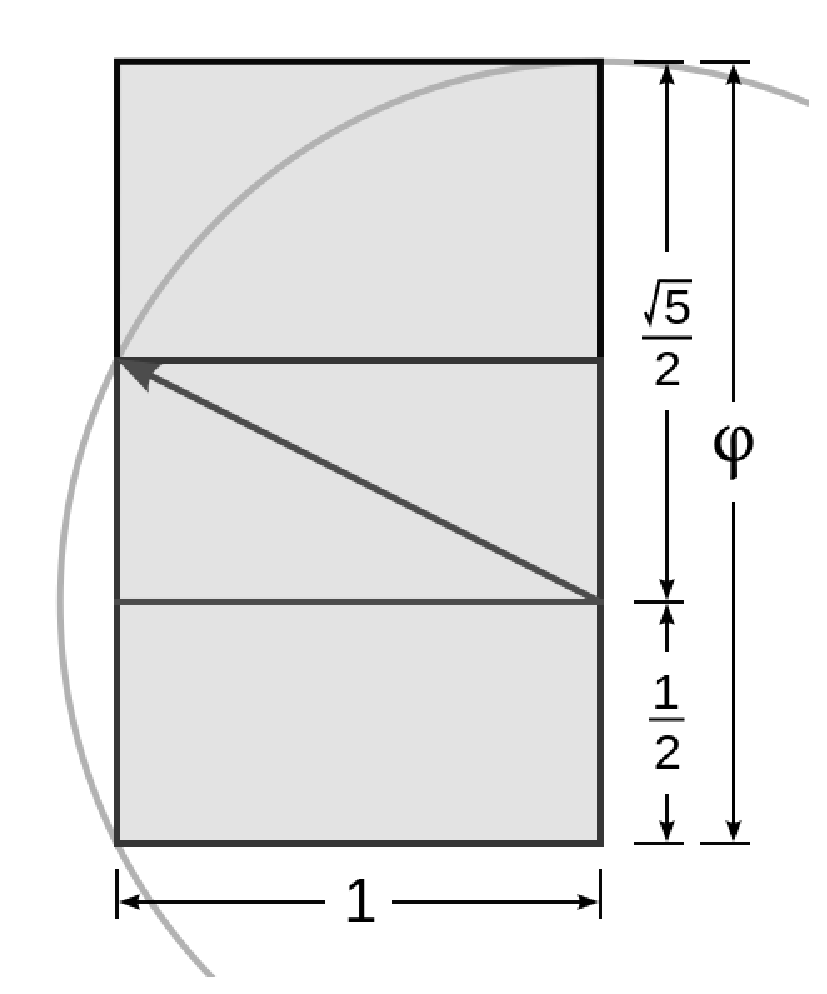
\includegraphics[scale=0.25]{images/construction}
   \caption{Una construcción con regla y compás del recángulo áureo.}
   \label{fig:construction}
\end{figure}

Hay varias expresiones curiosas del número $\varphi$. Puede expresarse por ejemplo como
la fracción continua 
\[
	\varphi=1+\cfrac{1}{1+\cfrac{1}{1+\cfrac{1}{1+\cdots}}}.
\]
También como el número trigonométrico 
$\varphi=2\cos(\pi/5)$ o 
como el límite
\[
	\varphi=\lim_{n\to\infty}\frac{F_n}{F_{n-1}},
\]
donde $F_n$ es el $n$-ésimo término de la sucesión 
\href{https://oeis.org/A000045}{A000045}.
de Fibonacci. 
Otra curiosa expresión para el número $\varphi$ es 
\[
	\varphi=\sqrt{1+\sqrt{1+\sqrt{1+\cdots}}}.
\]


\begin{exercise}
	Demuestre la veracidad de las expresiones del número $\varphi$ mencionadas
	en esta sección. 
\end{exercise}

Los rectángulos áureos aparecen en una tabla babilónica aproximadamente del año
850 a.C. que fue encontrada en Iraq en 1881. 

La publicación
en 1509 del libro \emph{Divina proportione} de Pacioli dio 
importancia al número $\varphi$,
especialmente entre artistas y arquitectos ya que los
rectángulos áureos son estéticamente más agradables que otros rectángulos. Hoy
en día es bastante fácil encontrarse con rectángulos áureos entre los objetos
que utilizamos comunmente. 

\section*{El método axiomático}

La intención original de Euclides fue la de deducir resultados a partir de
ciertas afirmaciones evidentes que llamó postulados (para nosotros, axiomas)
gracias al uso de ciertos principios básicos de la lógica. Estos libros de
Euclides constituyen el primer intento de derivar teoremas a partir de axiomas.
Según Heath, el método deductivo se le debe a Tales. 

Hoy en día nuestra forma de ver el método deductivo es levemente distinta.  El
método deductivo está basado en las leyes de la lógica y se compone de las
siguientes partes:
\begin{enumerate} 
	\item \emph{Términos primitivos}, que son ciertos elementos que no necesitan
			definirse tales como los puntos, las líneas y los planos de la
			geometría y las relaciones de incidencia entre ellos. No es
			importante el nombre que elijamos para estos elementos que no vamos
			a definir. 
		\item \emph{Axiomas o postulados}, que son ciertas afirmaciones acerca
			de los elementos primitivos, como bien podría ser el axioma que
			dice que dados dos puntos distintos existe una única línea recta
			que los contiene. Los axiomas se asumen verdaderos y no necesitan
			ser demostrados. 
		\item \emph{Teoremas}, que son simplemente las consecuencias lógicas de
			los axiomas.
\end{enumerate}

El rigor matemático de nuestro tiempo parece sugerir que el tratamiento
axiomático de Euclides no fue lo suficientemente riguroso. Sin embargo, no
tiene sentido mirar el texto de Euclides con nuestros ojos, hay que mirar la
matemática en perspectiva. En tiempos de Euclides el rigor matemático era
obviamente visto de forma completamente distinta. ¡Si la humanidad utilizó
durante dos mil años los libros de Euclides como libros de texto, seguro que no
fue por error o accidente! No parece apropiado criticar el rigor matemático
utilizado en los libros de Euclides después de recordar que fueron necesarios
dos mil años para entender cuáles eran los puntos de debilidad del tratado de
Euclides.

Veamos cuáles son los puntos donde hoy en día se critica el rigor matemático
del método axiomático de Euclides.  En los elementos de Euclides no existen los
términos primitivos, la lista de axiomas no es exhaustiva, algunas
demostraciones no están axiomáticamente justificadas, falta el uso de un cierto
principio de continuidad que garantice la existencia de ciertos puntos o líneas
que Euclides afirma que existen\dots Sí, nuestro rigor matemático se sentirá
levemente molesto por algunas cosas que encontramos en los libros de Euclides,
pero entre estas cosas hay una que se destaca notablemente. Una de las
diferencias fundamentales entre nuestra forma de ver el método axiomático y
aquella de Euclides está en el carácter que tienen los axiomas. ¡Los axiomas
elegidos no tienen por qué ser evidentes!  Hoy sabemos que hay otras geometrías
además de aquella de Euclides, y precisamente la existencia de estas otras
posibles geometrías no muestra que los axiomas elegidos pueden no ser
evidentes. ¿Acaso son evidentes las geometrías no euclidianas?

Si bien desde nuestro punto de vista moderno los axiomas impuestos por Euclides
tienen ciertas fallas, la matemática necesitó casi dos mil años para poder
encontrar fundamentos más precisos para la geometría. 

En el invierno de 1898
Hilbert dictó un curso en Gotinga sobre los fundamentos de la geometría. A
pedido de Klein, preparó notas poco tiempo después; notas que luego se
transformaron en un libro muy influyente, \emph{Grundlagen der Geometrie},
publicado en 1899, y que bien puede entenderse como una rectificación de la
geometría euclidiana. 

\section*{La fórmula de Herón}

\index{Fórmula!de Herón}
La fórmula de Herón nos dice que el área de un triángulo de lados $a$, $b$ y
$c$ está dada por la fórmula
\[
	\sqrt{s(s-a)(s-b)(s-c)},
\]
donde $s=\frac12(a+b+c)$. Esta fórmula puede demostrarse de muchas formas
distintas, por ejemplo con el teorema de Pitágoras o con la fórmula del coseno.

\begin{exercise}
	Utilice el teorema del coseno y demuestre la fórmula de Herón.
\end{exercise}

La fórmula aparece en el libro de Herón \emph{Métrica}, obra en tres volúmenes
donde Herón estudia las áreas de las superficies y los volúmenes de los
cuerpos. Estos libros estuvieron perdidos durante mucho tiempo,
hasta que fueron encontrados en 1896 por Schone en la ciudad de Constantinopla.
Una fórmula equivalente a la fórmula de Herón,
\[
	\frac14\sqrt{a^2b^2-\left(\frac{a^2+b^2-c^2}{2}\right)^2},
\]
fue encontrada en la matemática china y aparece en un libro publicado en 1247.

\index{Fórmula!de Arquímedes}
Se cree que Arquímedes conocía la fórmula de Herón pues entre sus escritos
figura el siguiente resultado: Supongamos que se tiene un triángulo $\Delta$ de
lados $q_1$, $q_2$ y $q_3$ y sean $Q_1=q_1^2$, $Q_2=q_2^2$ y $Q_3=q_3^2$.
Entonces 
\[
	16\times \textrm{área}(\Delta)^2=(Q_1+Q_2+Q_3)^2-2\times(Q_1^2+Q_2^2+Q_3^2).
\]

\begin{example}
	Consideremos en el plano el triángulo $\Delta$ con vértices en los puntos
	$(1,2)$, $(3,1)$ y $(0,0)$. Entonces
	\[
		16\times\textrm{área}(\Delta)=20^2-2\times(25+25+100)=400-2\times 150=100.
	\]
\end{example}

\index{Fórmula!de Brahmagupta}
La fórmula de Herón puede deducirse de una fórmula más general conocida como la
fórmula de Brahmagupta. Supongamos que se tiene un cuadrilátero de lados $a$,
$b$, $c$ y $d$ inscripto en círculo. Entonces el área del cuadrilátero es igual
a 
\[
	\sqrt{(s-a)(s-b)(s-c)(s-d)},
\]
donde $s=\frac12(a+b+c+d)$. 

\begin{exercise}
	Demuestre la fórmula de Herón a partir de la fórmula de Brahmagupta.
\end{exercise}

\begin{exercise}
	Demuestre la fórmula de Brahmagupta.
\end{exercise}

\section*{Trigonometría}

Hiparco fue el primero en compilar algo similar a una tabla trigonométrica y
por eso se lo conoce como ``el padre de la trigonometría''.  Poco tiempo
después Tolomeo tabuló las cuerdas para distintos ángulos y construyó una
verdadera tabla trigonométrica. La motivación era puramente práctica: la
astronomía requería la construcción de una tabla de cuerdas para distintos
arcos de una circunferencia. Gran parte de los descubrimientos de Tolomeo están
diseminadas a lo largo de sus escritos sobre astronomía.  La construcción de
Tolomeo se basa en la tabla comenzada por Hiparco y constituye una primera
versión de lo que hoy entendemos como trigonometría. Tolomeo utiliza polígonos
regulares de 3,4,5,6 y 10 lados y logra calcular las cuerdas de $36$, $60$,
$72$, $90$ y $120$ grados. Después de aplicar el teorema de Pitágoras obtiene
también las cuerdas de $108$ y $144$ grados. El uso de otros teoremas le
permite calcular otras cuerdas. Con la mente puesta en intentar obtener más
datos para su tabla de cuerdas, Tolomeo demuestra 
la igualdad trigonométrica 
\[
	\sin^2\left(\frac{x}{2}\right)=\frac{1-\cos x}{2}.
\]
y que la función $x\mapsto \sin x/x$ 
es decreciente para ciertos valores de $x$, resultado que era ya conocido,
aunque sin demostración, por Aristarco y Arquímedes.  Demuestra además lo que
conocemos como el teorema de Tolomeo, que afirma que si se tiene un
cuadrilátero de vértices A, B, C y D inscripto en un círculo tal como lo vemos
en la figura~\ref{fig:Tolomeo}, entonces
\[
	AC\times BD=AB\times CD+BC\times AD.
\]

\begin{figure}[h]
   \centering
   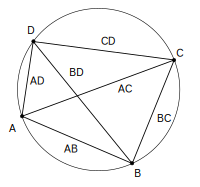
\includegraphics[scale=0.6]{images/tolomeo}
   \caption{El teorema de Tolomeo.}
   \label{fig:Tolomeo}
\end{figure}

\begin{exercise}
	Demuestre el teorema de Tolomeo.
\end{exercise}

Motivados por la astronomía, los árabes también tabularon tablas
trigonométricas hacia fines del siglo VIII. Ellos introdujeron las funciones
circulares y construyeron y perfeccionaron tablas para los valores de la
función seno.  

Grandes avances aparecieron en los siglos IX y X, donde por
ejemplo se logró perfeccionar las tablas de Tolomeo hasta lograr calcular
valores para la función seno con nueve decimales exactos. 

Los indios también tabularon tablas trigonométricas y lo hicieron tabulando
$\sin\theta$.  Medían ángulos en grados, minutos y segundos, ya que usaban la
base 60 de los babilónicos. Por eso, para ellos el valor máximo de la función
seno se alcanzaba aproximadamente en 3438:
\[
	360\times 60=21600=2\pi r
\]
de donde se deduce que $r$ debe ser aproximadamente igual a 3438. Utilizaban 
$3\frac{177}{1250}=3,1416$ como aproximación para el número $\pi$. 

Bhaskhara descubrió una sorprendente aproximación para la función seno, que
lamentablemente no es muy conocida. Si el ángulo $\theta$ se mide en grados y
está entre 0 y 180, se tiene
\[
	\sin\theta\sim \frac{r40(180-\theta)}{40500-\theta(180-\theta)}.
\]
Si traducimos esta fórmula al uso de radianes obtenemos
\[
	\sin x\sim\frac{16x(\pi-x)}{5\pi^2-4x(\pi-x)},\quad 0<x<\pi,
\]
fórmula que, tal como vemos en la figura~\ref{fig:baskhara} da una aproximación
asombrosamente buena.  

No sabemos cómo hizo Bhaskhara para encontrar tal
aproximación, hay muchas posibles explicaciones pero creo que ninguna resulta
del todo convincente. Para el interesado, mas información sobre esta
sorprendente aproximación y una demostración moderna de la fórmula puede
encontrarse en~\cite{MR1108101,MR2793182}.

\begin{figure}[h]
   \centering
   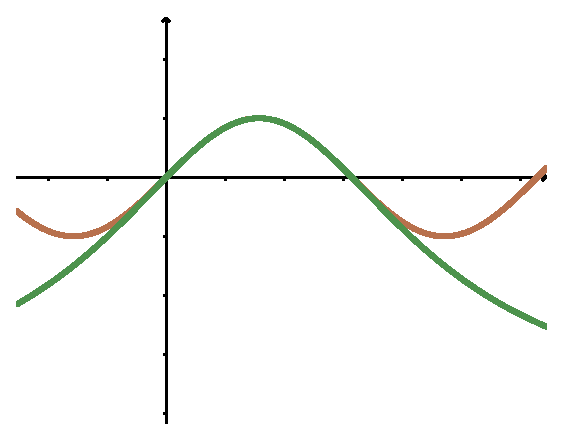
\includegraphics[scale=0.6]{images/baskhara}
   \caption{Una aproximación de Bhaskhara para la función seno.}
   \label{fig:baskhara}
\end{figure}

\index{Aproximación!de Palé}
Es interesante mencionar que la fórmula aproximada encontrada por Bhaskara es
muy similar a la que se obtendría si se utilizara la aproximación de Padé. En
1890, el matemático francés Padé desarrolló una técnica de aproximación de
funciones mediante funciones racionales: si $f$ es una función, $m\geq0$ y
$n\geq1$, se aproxima la función $f$ por una expresión racional de la forma
\[
	g(x)=\frac{a_0+a_1x+a_2x^2+\cdots+a_mx^m}{b_0+b_1x+b_2x^2+\cdots+b_nx^n},
\]
donde los coeficientes $a_0,\dots,a_m$ y $b_0\dots,b_n$ se calculan para que
\[
	f(0)=g(0),\quad
	f'(0)=g'(0),\quad
	f''(0)=g''(0),\quad
	\dots
	\quad
	f^{(m+n)}(0)=g^{(m+n)}(0).
\]
Para mostrar qué tan buena puede llegar a ser esta aproximación concebida por
Palé, mencionamos que la función exponencial $e^x$ puede aproximarse fabulosamente
bien en el intervalo $-1/2\leq x\leq 1/2$ por la función racional
\[
	\frac{120+60x+12x^2+x^3}{120-60x+12x^2-x^3}.
\]

Las aproximaciones de Padé son en general muy buenas y tienen muchas
aplicaciones que involucran cálculos computacionales, ver por
ejemplo~\cite{MR1383091}.  

La idea de aproximar funciones por funciones
racionales había sido ya considerada por Frobenius en un trabajo publicado en
1881.  

Alrededor del año 100 a. C. Menelao publicó un tratado en tres volúmenes donde
aparecen por primera vez los triángulos esféricos y algunas de sus propiedades
más importantes, permitiéndonos reconocer las similitudes y las diferencias que
tienen los triángulos esféricos con los triángulos de la geometría clásica de
Euclides.  Podemos ver un triángulo esférico en la figura~\ref{fig:esferico}.

\begin{figure}[h]
   \centering
   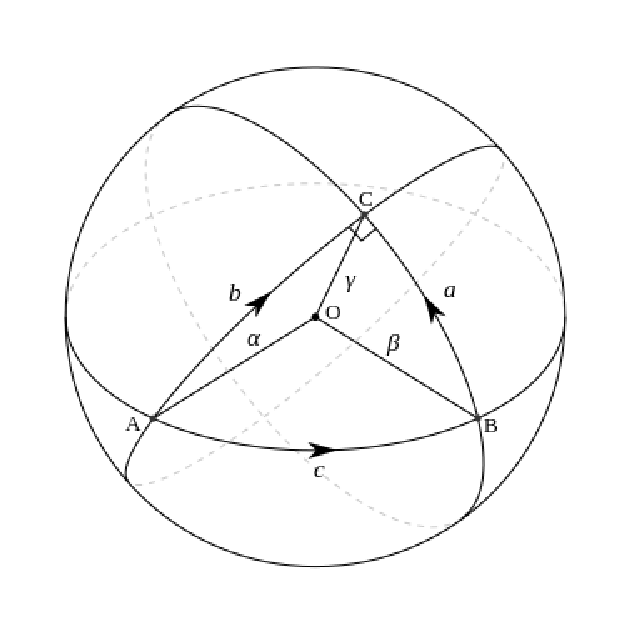
\includegraphics[scale=0.4]{images/esferico}
   \caption{Un triángulo esférico.}
   \label{fig:esferico}
\end{figure}

\index{Teorema!de Menelao}
En el tercero de estos libros aparecen dos resultados que hoy conocemos como teoremas de
Menelao. Estos teoremas no son sino dos versiones, una para la geometría plana y otra para
la geometría esférica, de un mismo resultado sobre triángulos.  En su versión
relativa a la geometría plana, el teorema de Menelao afirma que si se tiene un
triángulo como el que vemos en la figura~\ref{fig:Menelao}, donde vemos una
recta que corta al segmento AB en el punto E, al segmento CB en D y a la
prolongación de la línea AB en el punto F, entonces 
\[
	\frac{EA}{EC}\frac{DC}{DB}\frac{FB}{FA}=1.
\]

\begin{figure}[h]
   \centering
   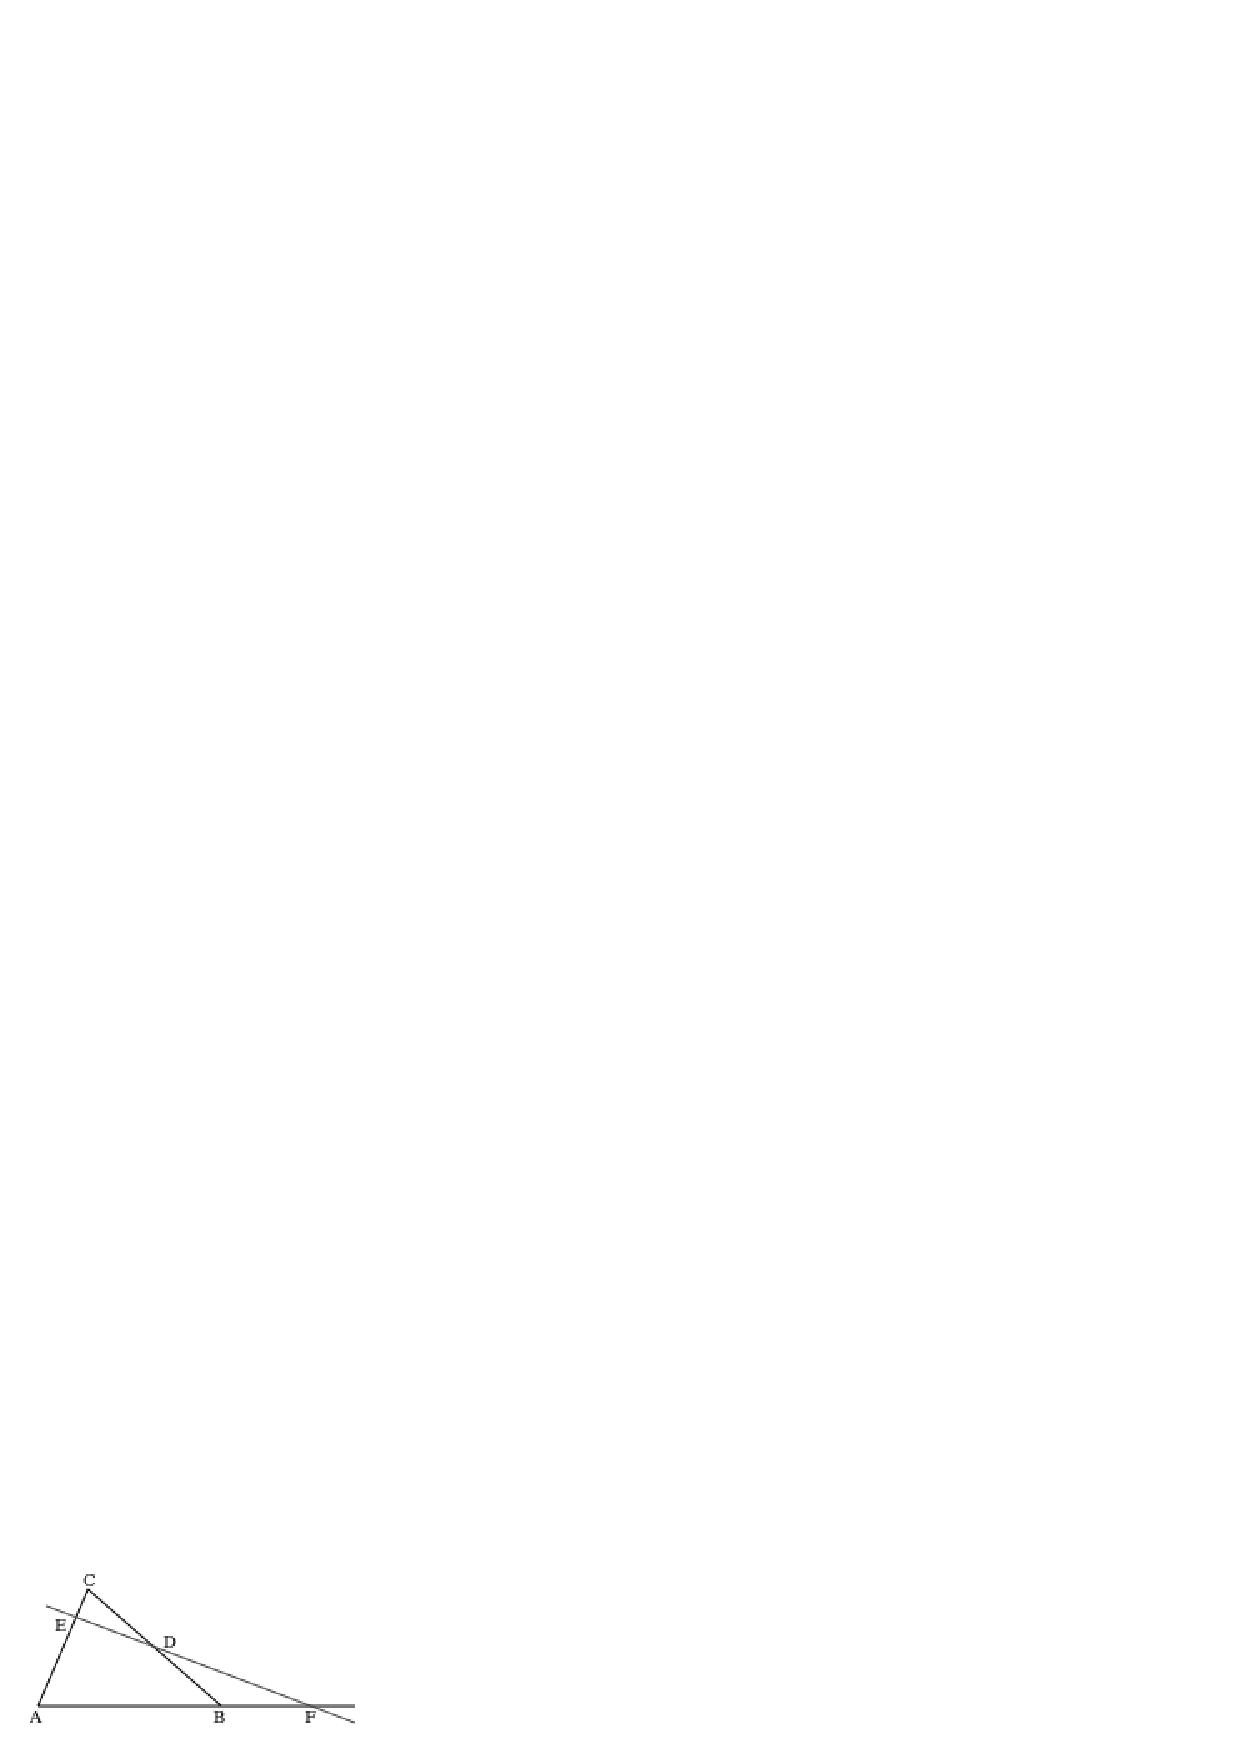
\includegraphics[scale=0.7]{images/menelao}
   \caption{El teorema de Menelao.}
   \label{fig:Menelao}
\end{figure}

\begin{exercise}
	Demuestre el teorema de Menelao.
\end{exercise}

Si bien este resultado de Menelao tiene un análogo en geometría esférica, no
toda la geometría clásica puede adaptarse al contexto esférico. De hecho, tal
como demostró Menelao en el primer volumen, la suma de los ángulos interiores
de un triángulo esférico es siempre mayor a $180$ grados. 

\section*{Las cónicas de Apolonio}

\index{Cónicas}
\index{Elipse}
\index{Hipérbola}
\index{Parábola}
Las \textbf{cónicas} son aquellas curvas que se obtienen al cortar un cono
circular con un plano, tal como vemos en la figura~\ref{fig:conicas}. Las
cónicas son entonces hipérbolas, elipses o parábolas. Vemos una hipérbola en la
figura~\ref{fig:hiperbola}.

\begin{figure}[h]
   \centering
   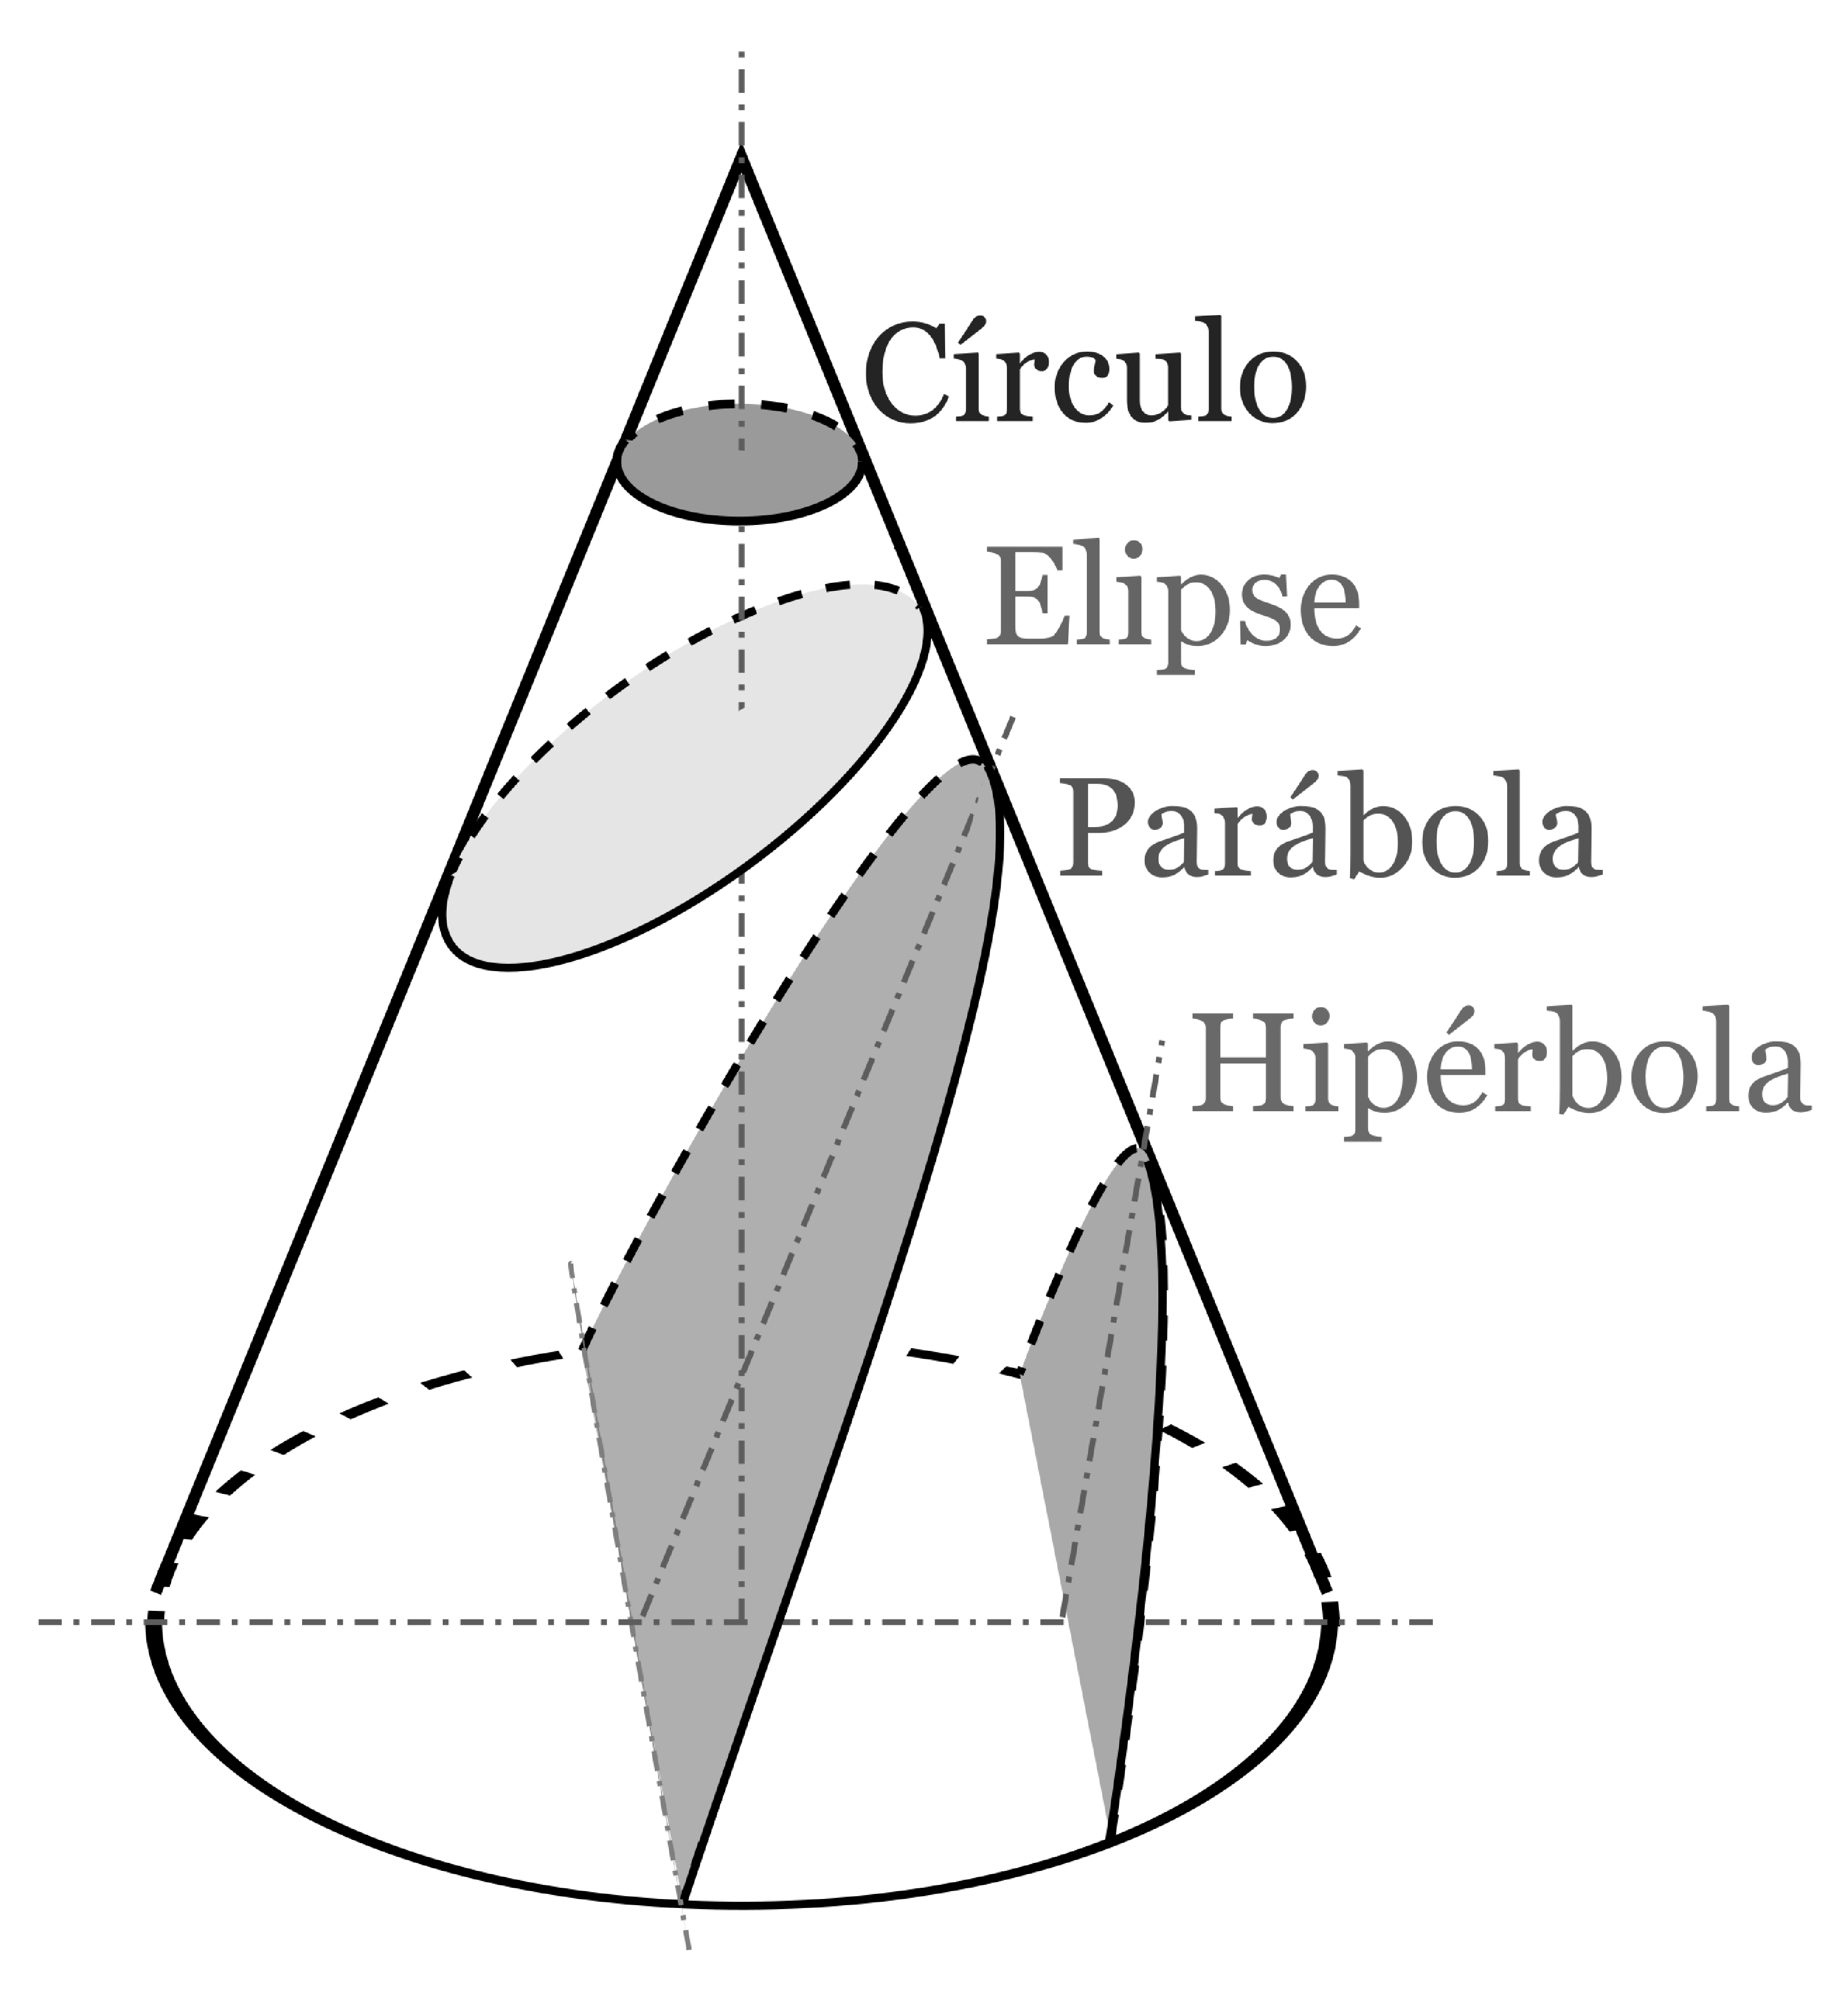
\includegraphics[scale=0.05]{images/conicas}
   \caption{Cónicas.}
   \label{fig:conicas}
\end{figure}

\begin{figure}[h]
   \centering
   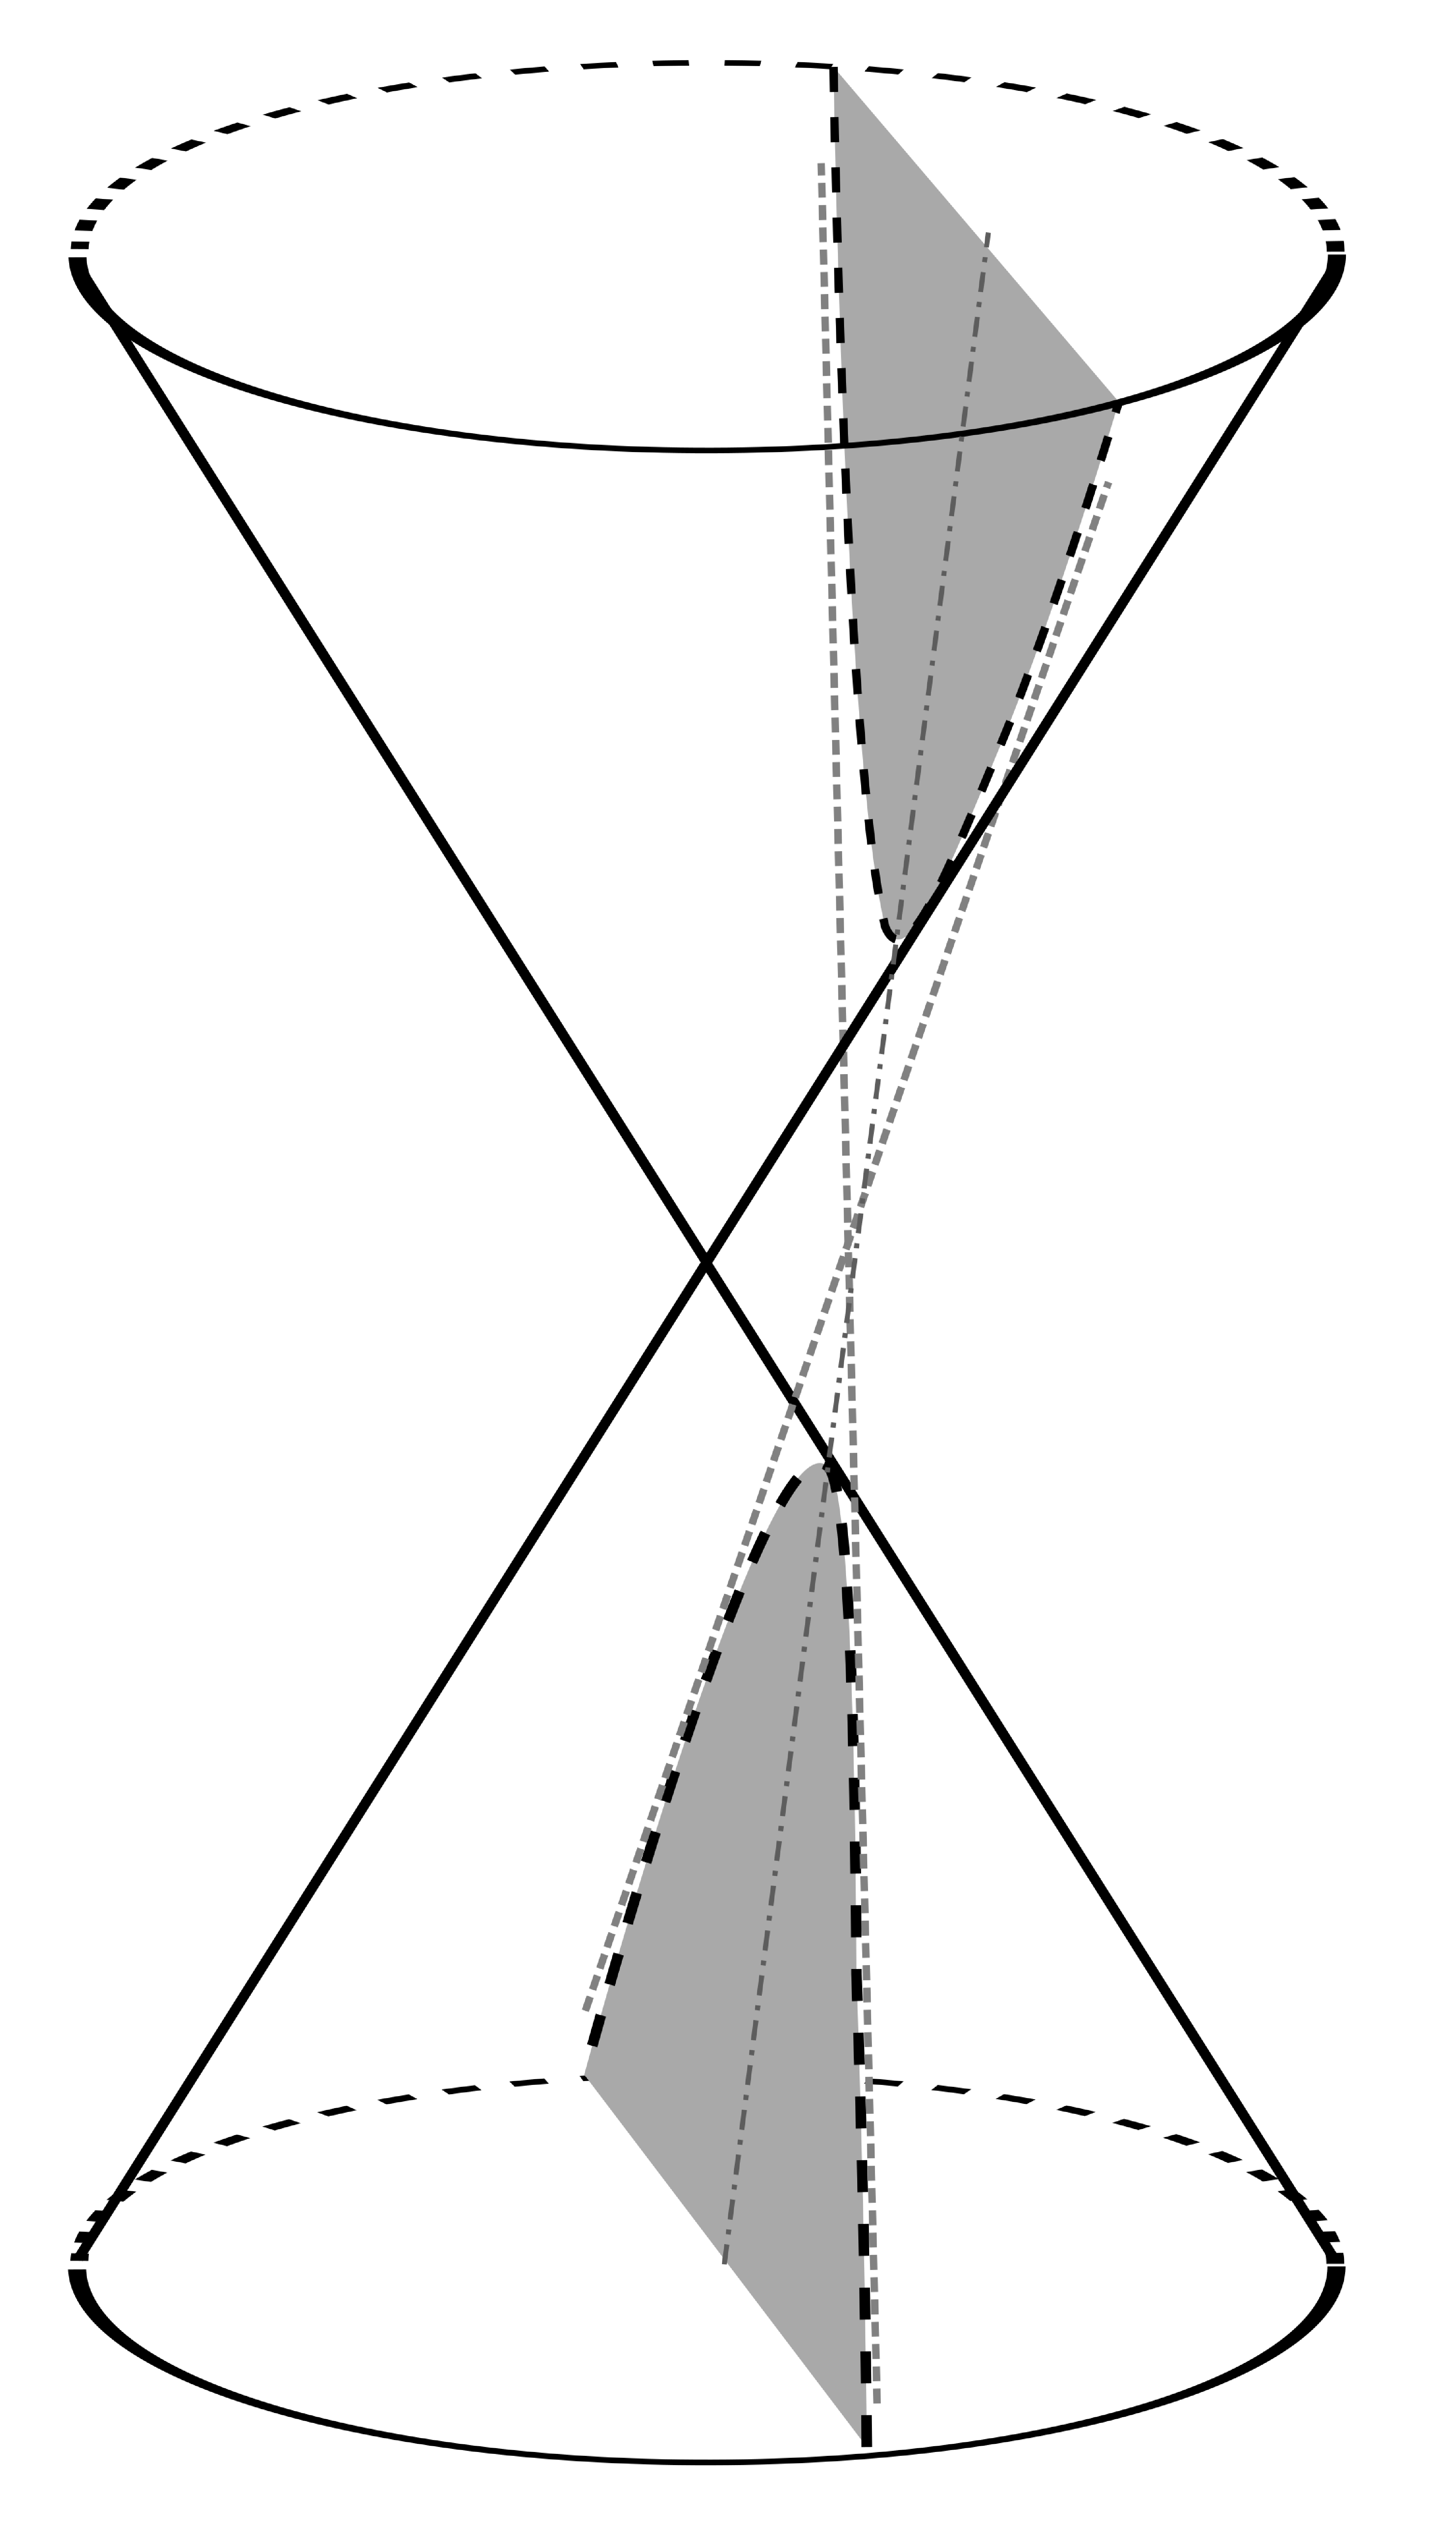
\includegraphics[scale=0.04]{images/hiperbola}
   \caption{Una hipérbola.}
   \label{fig:hiperbola}
\end{figure}

Hoy sabemos que podemos representar cónicas mediante ecuaciones. La
expresión 
\[
	\frac{x^2}{a^2}-\frac{y^2}{b^2}=1
\]
es la ecuación de una hipérbola, la expresión 
\[
	\frac{x^2}{a^2}+\frac{y^2}{b^2}=1
\]
es la ecuación de una elipse y la expresión 
\[	
	y=ax^2
\]
es la ecuación de una parábola. 

Se cree que las cónicas fueron inventadas por Menecmo en épocas de Alejandro
Magno. Originalmente Menecmo utilizó las cónicas para reformular (y en algún
sentido resolver) el famoso problema de la duplicación del cubo. En nuestra
notación, el problema de la duplicación del cubo puede reformularse como el
problema de encontrar la intersección de la parábola $y=\frac12x^2$ con la
hipérbola $xy=1$, ya que esto implica encontrar un $x$ tal que $x^3=2$. Los
griegos aparentemente nunca discutieron sobre los instrumentos necesarios
para dibujar cónicas, aunque sí aceptaron la solución propuesta por Menecmo.
Las ideas de Menecmo sugieren la existencia de un instrumento que resulta ser
una generalización del compás, este instrumento, en forma independiente,
aparece en la matemática árabe del siglo XI. 

El estudio profundo de las cónicas y sus propiedades fhe hecho por Apolonio,
alrededor del año 200 a. C.  Apolonio escribió ocho libros, de los que
conocemos solamente los primeros cuatro en versión original y los tres
restantes mediante traducciones árabes. En la introducción Apolinio escribe
algo que nos permite deducir cómo es que la matemática se transmitía en aquella
época. Los primeros cuatro libros sobre cónicas están dedicados a Eudemo.  Por
la introducción sabemos que Apolinio puso el segundo libro en manos de su hijo
para que él entregara el volumen a Eudemo. Allí le pide que lo lea con cuidado
y que divulgue los resultados allí contenidos a todo aquel que muestre interés.
Pide además a Eudemo que le muestre el libro al geómetra Filónides si llegara a
presentarse la oportunidad. 

%Aparentemente, el geómetra Neucrates tenía en sus manos una versión preliminar
%del tratado de Apolonio. 

Según Apolonio, los primeros cuatro libros forman una introducción elemental,
los restantes versan sobre tópicos más avanzados.  Se estudian propiedades
básicas de las cónicas en el primer libro. En el segundo, se estudian la
hipérbola y sus asíntotas. En el tercero aparecen los focos de la elipse y de
la hipérbola, no así el de la parábola, quizá porque Apolonio no lo consideró
suficientemente interesante, y aparecen además propiedades relativas a los
triángulos y a los cuadrados inscritos y circunscritos (muy posiblemente, estas
propiedades sean las que utilizó Apolonio para estudiar el ``problema de las
tres rectas'' y el ``problema de las cuatro rectas'', algo que aparecerá
después en los trabajos de Pappus). Aparecen además ciertas propiedades métricas
de las cónicas, propiedades que hoy suelen pertenecer a cursos de geometría
proyectiva. Por último, en el cuarto libro se estudian intersecciones y contacto
entre cónicas. En este volumen Apolonio demuestra que dos cónicas no pueden
tener más de cuatro puntos en común. En el quinto libro se estudian las
distancias máxima y mínima de un punto a los puntos de una cónica, resultados
que le dieron fama a Apolonio como geómetra. El sexto libro es quizá menos
importante que el anterior dado que el objetivo principal es el de ordenar y
completar trabajos anteriores, tales como el tratado de Arquímedes sobre
conoides y esferoides. En el libro siete se estudian máximos y mínimos de
ciertas funciones de los diámetros de las cónicas. 

%De hecho, Apolonio está tan ligado a las cónicas como Euclides lo está con sus elementos. 
%Apolonio

Dado que no disponían del álgebra, los griegos no
pudieron estudiar sistemáticamente curvas de grado superior. Sin embargo, sí
fueron capaces de estudiar ciertas curvas particulares sin necesidad de
utilizar ecuaciones que las definan. Un ejemplo notable es la cisoide de
Diocles. 

\section*{Algunas curvas algebraicas}

\index{Curva!algebraica}
Como los griegos no disponían del álgebra, no pudieron profundizar sus
conocimientos sobre curvas, aunque sí pudieron estudiar algunas curvas
algebraicas particulares. Una curva algebraica es una curva dada por los ceros
de un polinomio de dos variables.  Para una digresión histórica sobre la teoría
de curvas algebraicas, referimos al primer capítulo del libro de Brieskorn y
Kn\"{o}rrer \cite{MR2975988}.

\index{Cisoide de Diocles}
Veamos algunos ejemplos de las curvas consideradas en la matemática griega. 
Diocles concibió la curva de hoy conocemos como \emph{cisoide de Diocles} y observó que
esta curva permite duplicar el cubo. Podemos ver una representación gráfica de
esta curva en la figura~\ref{fig:cisoide}. En nuestra notación, esta curva
está representada por la ecuación
\[
	y^2(1+x)=(1-x)^3.
\]

\begin{figure}
   \centering
   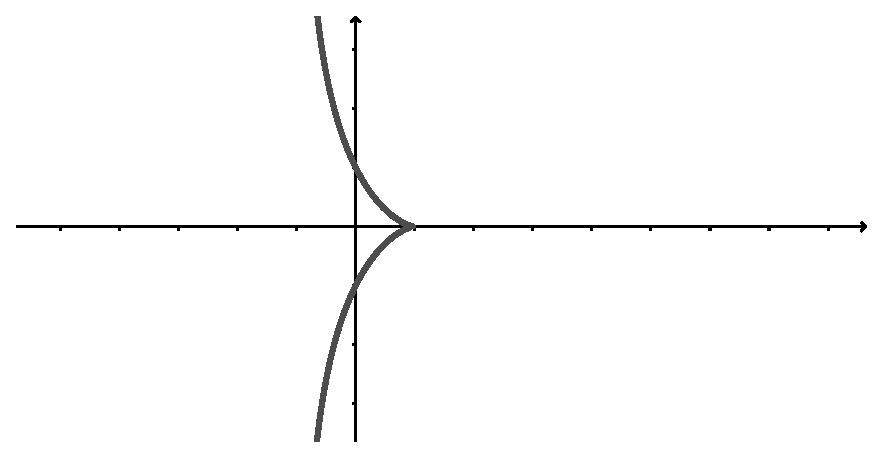
\includegraphics[scale=0.3]{images/cisoide}
   \caption{La cisoide de Diocles.}
   \label{fig:cisoide}
\end{figure}

\index{Toro}
\index{Secciones espíricas}
Los matemáticos griegos conocían algunas superficies. Una de las superficies
que estudiaron es el toro, que es una superficie de revolución tal como la que
podemos ver en la figura~\ref{fig:toro}. 

\begin{figure}
   \centering
   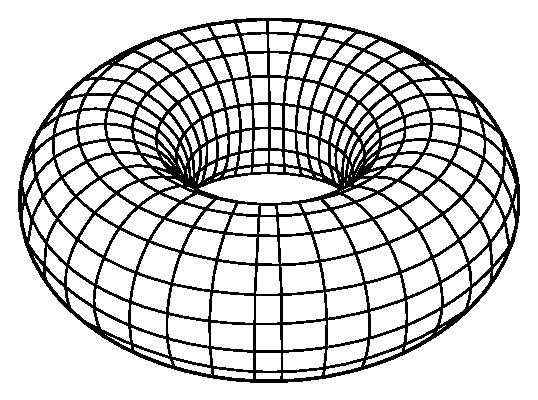
\includegraphics[scale=0.3]{images/toro}
   \caption{El toro.}
   \label{fig:toro}
\end{figure}

Perseo estudió las curvas que se obtienen al cortar el toro
con planos paralelos al eje de rotación, estas curvas se conocen como 
\emph{curvas espíricas}. La ecuación de estas curvas está dada por
\[
	(x^2+y^2)^2=dx^2+ey^2+f.
\]

\begin{figure}
   \centering
   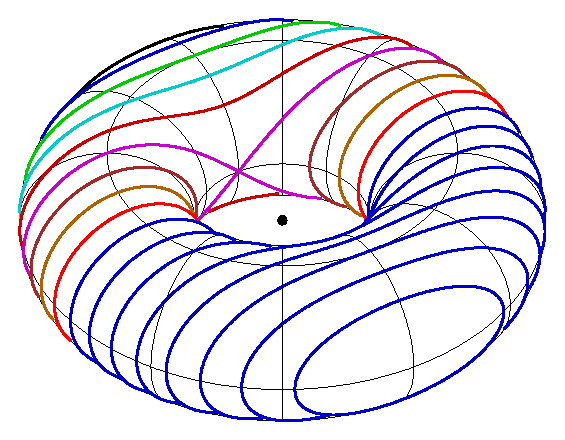
\includegraphics[scale=0.3]{images/spiric}
   \caption{Las curvas espíricas.}
   \label{fig:spiric}
\end{figure}



\index{Lemniscata de Bernoulli}
Algunas de estas curvas fueron redescubiertas en el
siglo XVII gracias a la geometría analítica de Descartes. Un ejemplos notable 
el de la \emph{lemniscata de Bernoulli}, descubierta en 1694 por Jakov Bernoulli. La ecuación 
de esta curva es 
\[
	(x^2+y^2)^2=x^2-y^2
\]
y podemos ver una representación gráfica en la figura~\ref{fig:lemniscata}.

\begin{figure}
   \centering
   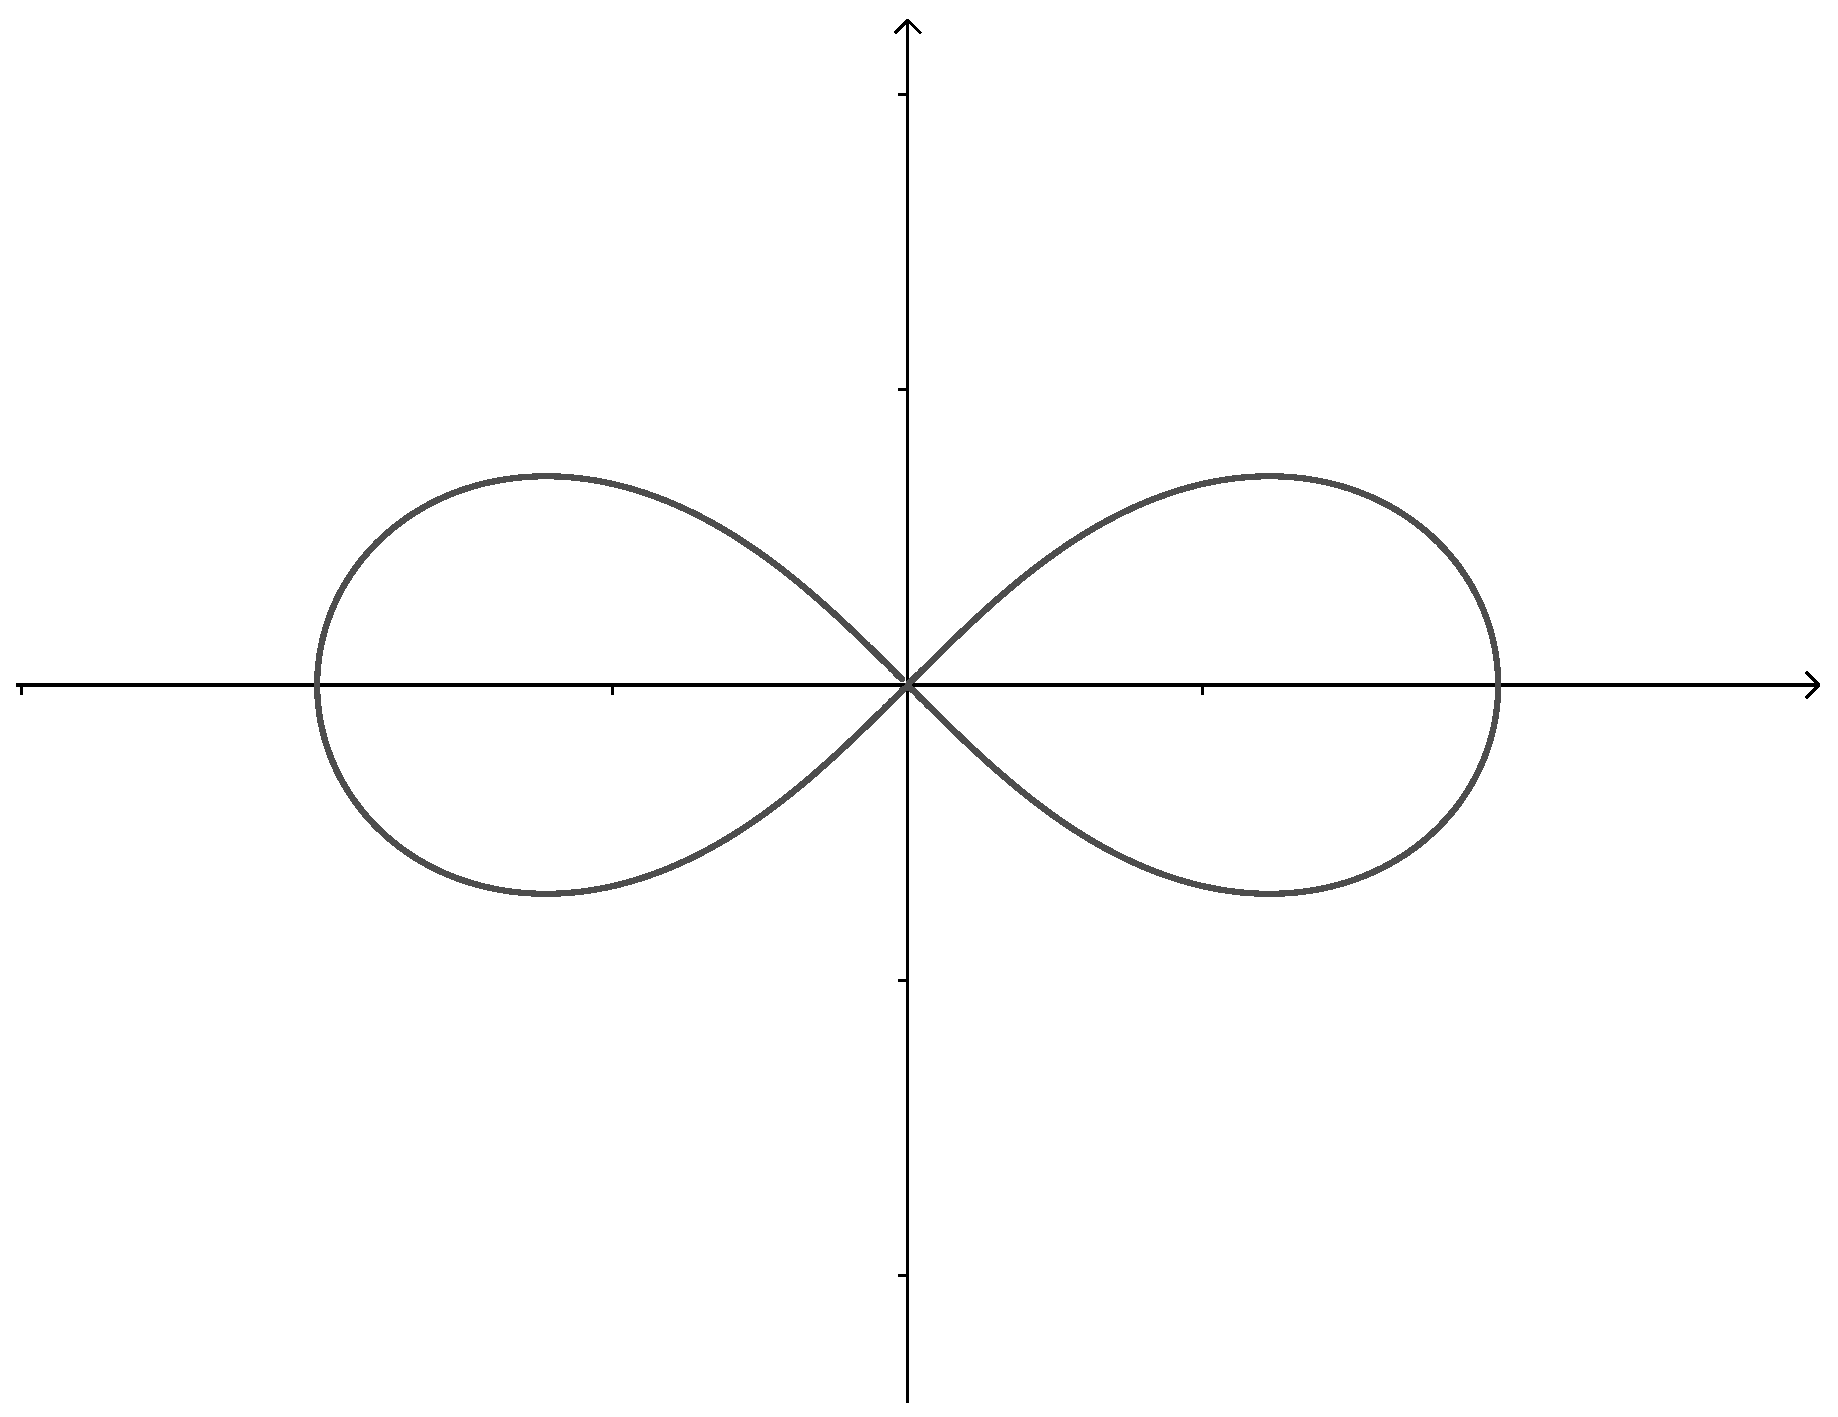
\includegraphics[scale=0.2]{images/lemniscata}
   \caption{La Lemniscata de Bernourlli.}
   \label{fig:lemniscata}
\end{figure}
 
\index{Óvalos de Cassini}
Otro ejemplo es el de los \emph{óvalos de Cassini}, que vemos en la
figura~\ref{fig:Cassini}, y que el astrónomo propuso para reemplazar a las
elipses de Kepler que describen las órbitas planetarias. La lemniscata
es un ejemplo de óvalo de Cassini.

\begin{figure}
   \centering
   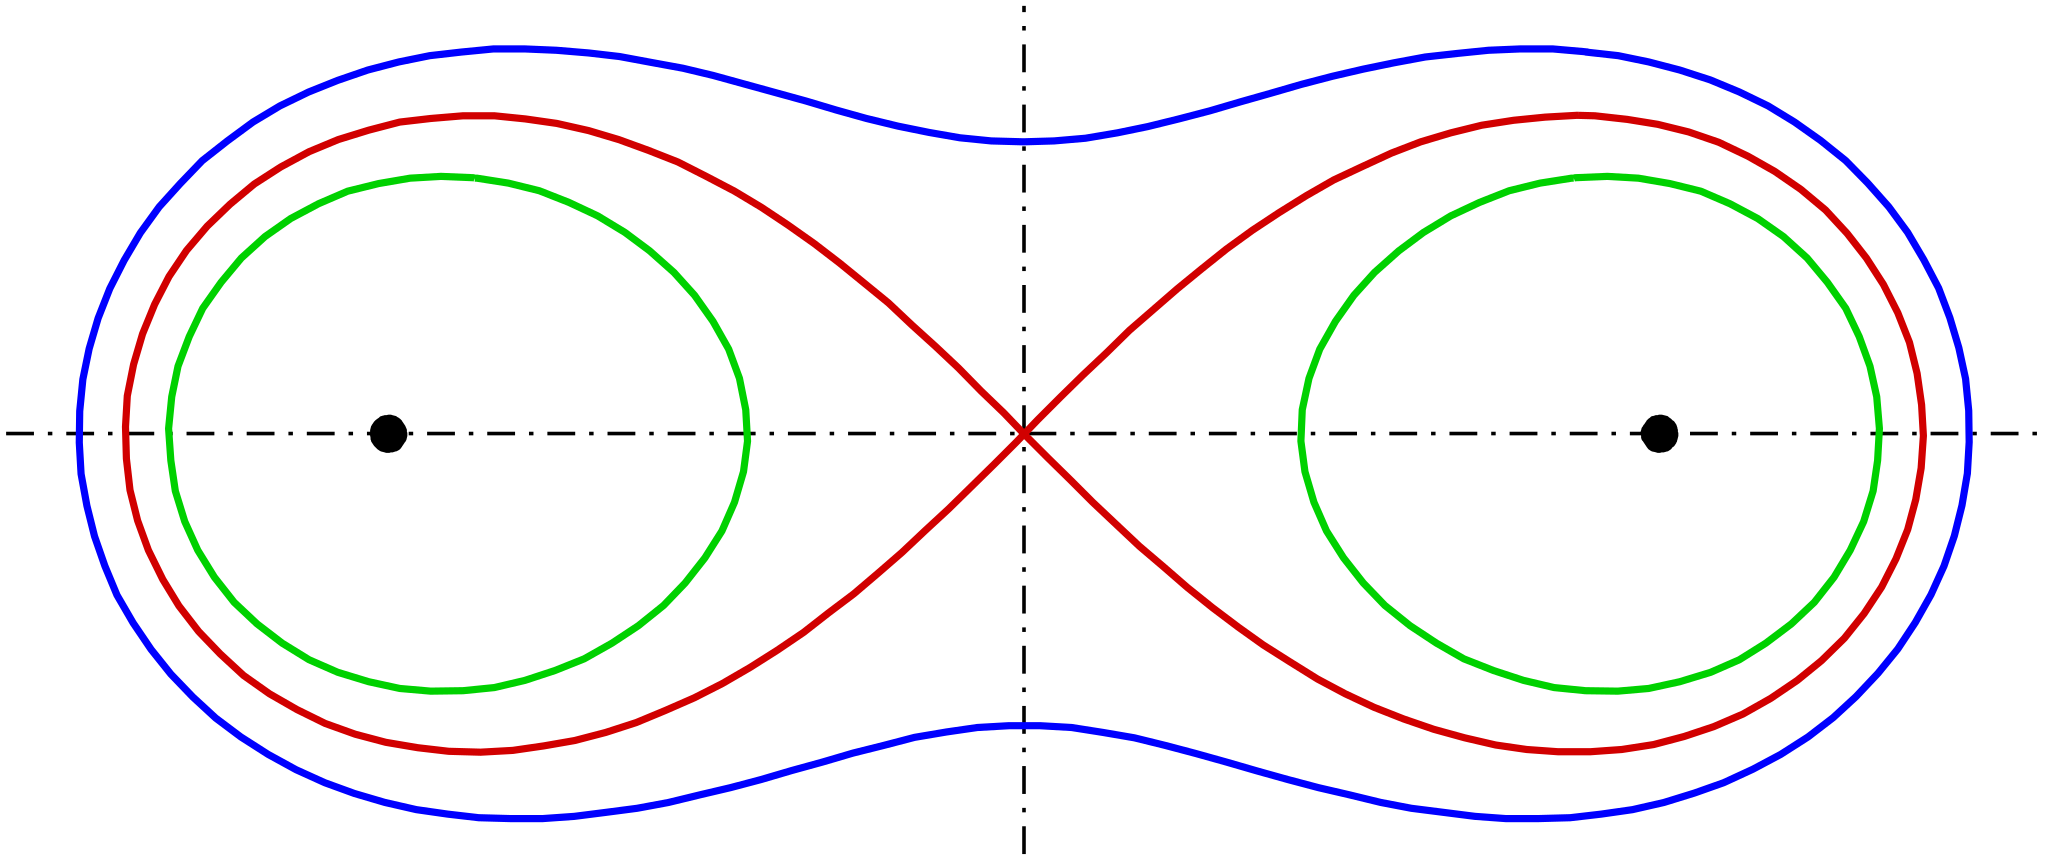
\includegraphics[scale=0.5]{images/cassini}
   \caption{Los óvalos de Cassini.}
   \label{fig:Cassini}
\end{figure}

\index{Epiciclos de Ptolomeo}
\index{Cardioide}
Otra familia de curvas estudiadas por la matemática griega es la de los
epiciclos de Ptolomeo. Estas curvas también tienen sus orígenes en la
astronomía, ya que eran los candidatos naturales a describir las órbitas
planetarias. Un ejemplo de estas curvas es el de la \emph{cardioide} de ecuación
\[
	(x^2+y^2-1)^2=4( (x-1)^2+y^2)
\]
que vemos en la figura~\ref{fig:cardioide}.

\begin{figure}
   \centering
   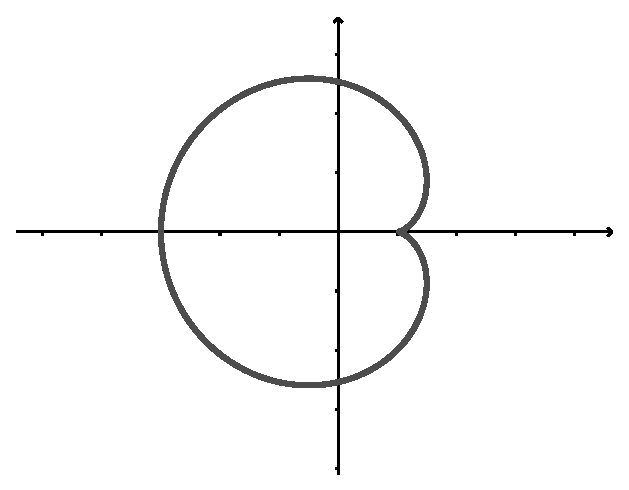
\includegraphics[scale=0.5]{images/cardioid}
   \caption{La cardioide.}
   \label{fig:cardioide}
\end{figure}
 
